\section{Sallen-Key}

Se iniciará el estudio y diseño de celdas con la implementación mediante una celda de tipo \emph{Sallen Key} de un filtro pasa-bajos aproximado con Butterworth. Se realizará un análisis teórico de la celda y sus características, el diseño de la misma para cumplir con los parámetros calculados previamente usando la aproximación, y simulaciones en LTSpice para observar el cumplimiento del filtro y el efecto de las variaciones de los componentes pasivos. 

\subsection{Cálculo de función transferencia por aproximación de Butterworth}

A partir de las características especificadas por la plantilla de la tabla \ref{table:Plantilla} y representadas en la figura \ref{fig:Plantilla}, se calculó la función transferencia mediante la aproximación de Butterworth. Observando las frecuencias límite para la banda de paso y la de atenuación, se denota que se trata de un filtro \emph{pasa-bajos}. La aproximación empleada resulta conveniente cuando se quiere asegurar la mayor planicie posible en la banda de paso y que la transferencia sea monótonamente decreciente. 

% Please add the following required packages to your document preamble:
% \usepackage[table,xcdraw]{xcolor}
% If you use beamer only pass "xcolor=table" option, i.e. \documentclass[xcolor=table]{beamer}
\begin{table}[H]
\centering
\begin{tabular}{|
>{\columncolor[HTML]{C0C0C0}}c |c|}
\hline
$f_{p}$  & 3300Hz  \\ \hline
$f_{a}$  & 15600Hz \\ \hline
$A_{p}$  & 3dB      \\ \hline
$A_{a}$  & 40dB     \\ \hline
$\left | Z_{in}(f) \right |$ & $\geq 50k \Omega $      \\ \hline
\end{tabular}
    \label{table:Plantilla}
\end{table}

\begin{figure}[H]
    \centering
    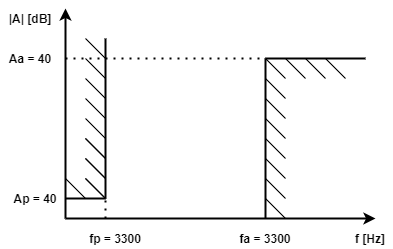
\includegraphics[width= 0.5\textwidth]{../Ejercicio2-DisenoDeCeldas/1CeldaSallenKey/images/plantilla.png}
    \caption{Plantilla desnormalizada}
    \label{fig:Plantilla}
\end{figure}

Partiendo de la expresión del cuadrado del módulo de la función transferencia \ref{eq:SK1}, se busca cumplir que las que las primeras $2n − 1$ derivadas del módulo de la transferencia se anulen en $w=0$. Para ello, se determinan los parámetros $\varepsilon$ y el orden del filtro. 

\begin{equation}
        \left | H(jw_{n}) \right |^{2} = \frac{1}{1+\varepsilon ^{2}w_{n}^{2}}
    \label{eq:SK1}
\end{equation}

\begin{equation}
        \varepsilon = \sqrt{10^{\frac{A_{p}(dB)}{10}}-1} \Rightarrow \varepsilon = 1
    \label{eq:SK2}
\end{equation}

\begin{equation}
        n = \left \lceil  \frac{\log \left ( \frac{10^{\frac{A_{a}(dB)}{10}}-1}{\varepsilon ^{2}} \right )}{2\cdot \log \left (\frac{w_{a}}{w_{p}} \right )} \right \rceil \Rightarrow n = \left \lceil  \frac{\log \left ( 10^{4}-1 \right )}{2\cdot \log \left (4,7272 \right )} \right \rceil = \left \lceil 2.964664 \right \rceil \Rightarrow n = 3 
    \label{eq:SK3}
\end{equation}


A partir del orden del filtro, se obtiene el polinomio de Butterworth que fija la ubicación normalizada de los polos. Se obtiene así la función transferencia normalizada correspondiente a un filtro pasa-bajos a implementar luego con un filtro activo. 


\begin{equation}
        H_{N}(s) = \frac{1}{(s+1)(s^{2}+s+1)}
    \label{eq:SK4}
\end{equation}

Donde la función transferencia desnormalizada se obtiene reemplazando $s\rightarrow \frac{s}{w_{p}}$. Se observa de \ref{eq:SK4} que el factor de calidad de la función de segundo orden es Q=1.

$$w_{p} = 2 \pi 3300 Hz = 20734.5 \frac{rad}{s}$$

\begin{figure}[H]
    \centering
    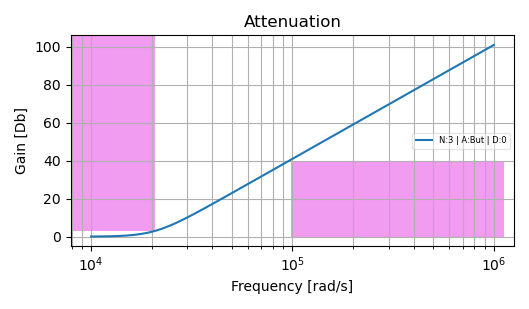
\includegraphics[width= 0.5\textwidth]{../Ejercicio2-DisenoDeCeldas/1CeldaSallenKey/images/AtenuacionButter.png}
    \caption{Butterworth orden 3}
    \label{fig:butter3}
\end{figure}


\begin{figure}[H]
    \centering
    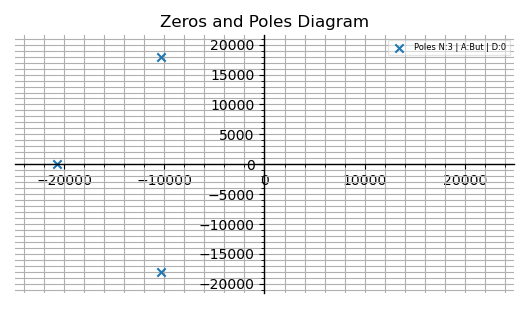
\includegraphics[width= 0.5\textwidth]{../Ejercicio2-DisenoDeCeldas/1CeldaSallenKey/images/PolesButter.png}
    \caption{Ubicación de polos polinomio de Butterworth}
    \label{fig:Plantilla}
\end{figure}

\subsection{Circuito a implementar}

Para la implementación de la función transferencia calculada, se segmentará el filtro en etapas que conectadas en cascada permitirán obtener el comportamiento deseado. Esto es posibilitado con la utilización de filtros activos, los cuales cuentan con una impedancia de salida muy baja que evita cargar la etapa siguiente, de modo que cada etapa puede considerarse prácticamente aislada de las demás, pudiendo calibrarse independientemente de ser necesario. Este enfoque de diseño proyecta un atractivo sobre las llamadas \textbf{celdas}, ya que proveen una forma casi estandarizada de implementar etapas de un filtro de segundo orden de determinadas características. 

Al implementar un diseño en cascada es importante cuidar el orden de conexión de las celdas. Si bien matemáticamente el orden de implementación es irrelevante, la conexión de las celdas puede tener algunas limitaciones. Por un lado, para evitar pérdida en el rango dinámico del filtro y la posibilidad de saturación de la señal en las etapas con un Q mas alto (y por lo tanto posibilidad de amplificación), se recomienda conectar las etapas de menor a mayor Q. Sin embargo, si se desea proteger del ruido interno del filtro, el cual puede causar inconvenientes con las etapas de Q alto, es conveniente ubicar las etapas de mayor Q al principio de la conexión. Vale destacar que, sin embargo, no se espera ninguno de estos inconvenientes en la implementación del filtro calculado ya que se cuenta con una única instancia de segundo orden.

Siguiendo el enfoque de diseño en cascada, se implementará el filtro pasa-bajos de tercer orden separándolo en dos etapas: la inicial de primer orden empleando un \textbf{circuito RC con buffer} a su salida y la segunda mediante una \textbf{celda Sallen-Key Low Pass}. Se realizará el análisis y diseño de cada instancia. 

\begin{figure}[H]
    \centering
    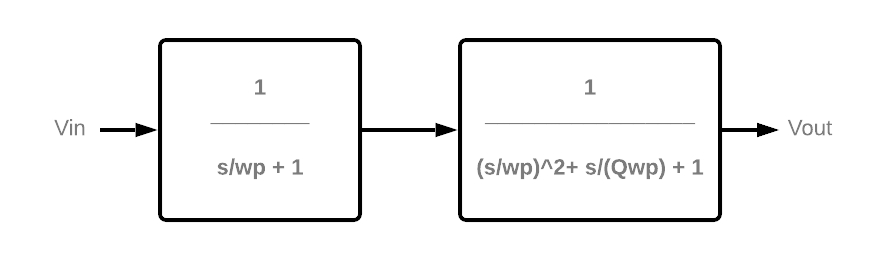
\includegraphics[scale = 0.4]{../Ejercicio2-DisenoDeCeldas/1CeldaSallenKey/images/Etapas.png}
    \caption{Diagrama de etapas en cascada.}
    \label{fig:etapas}
\end{figure}


\subsection{Celda de primer orden: Análisis}

\begin{figure}[H]
    \centering
    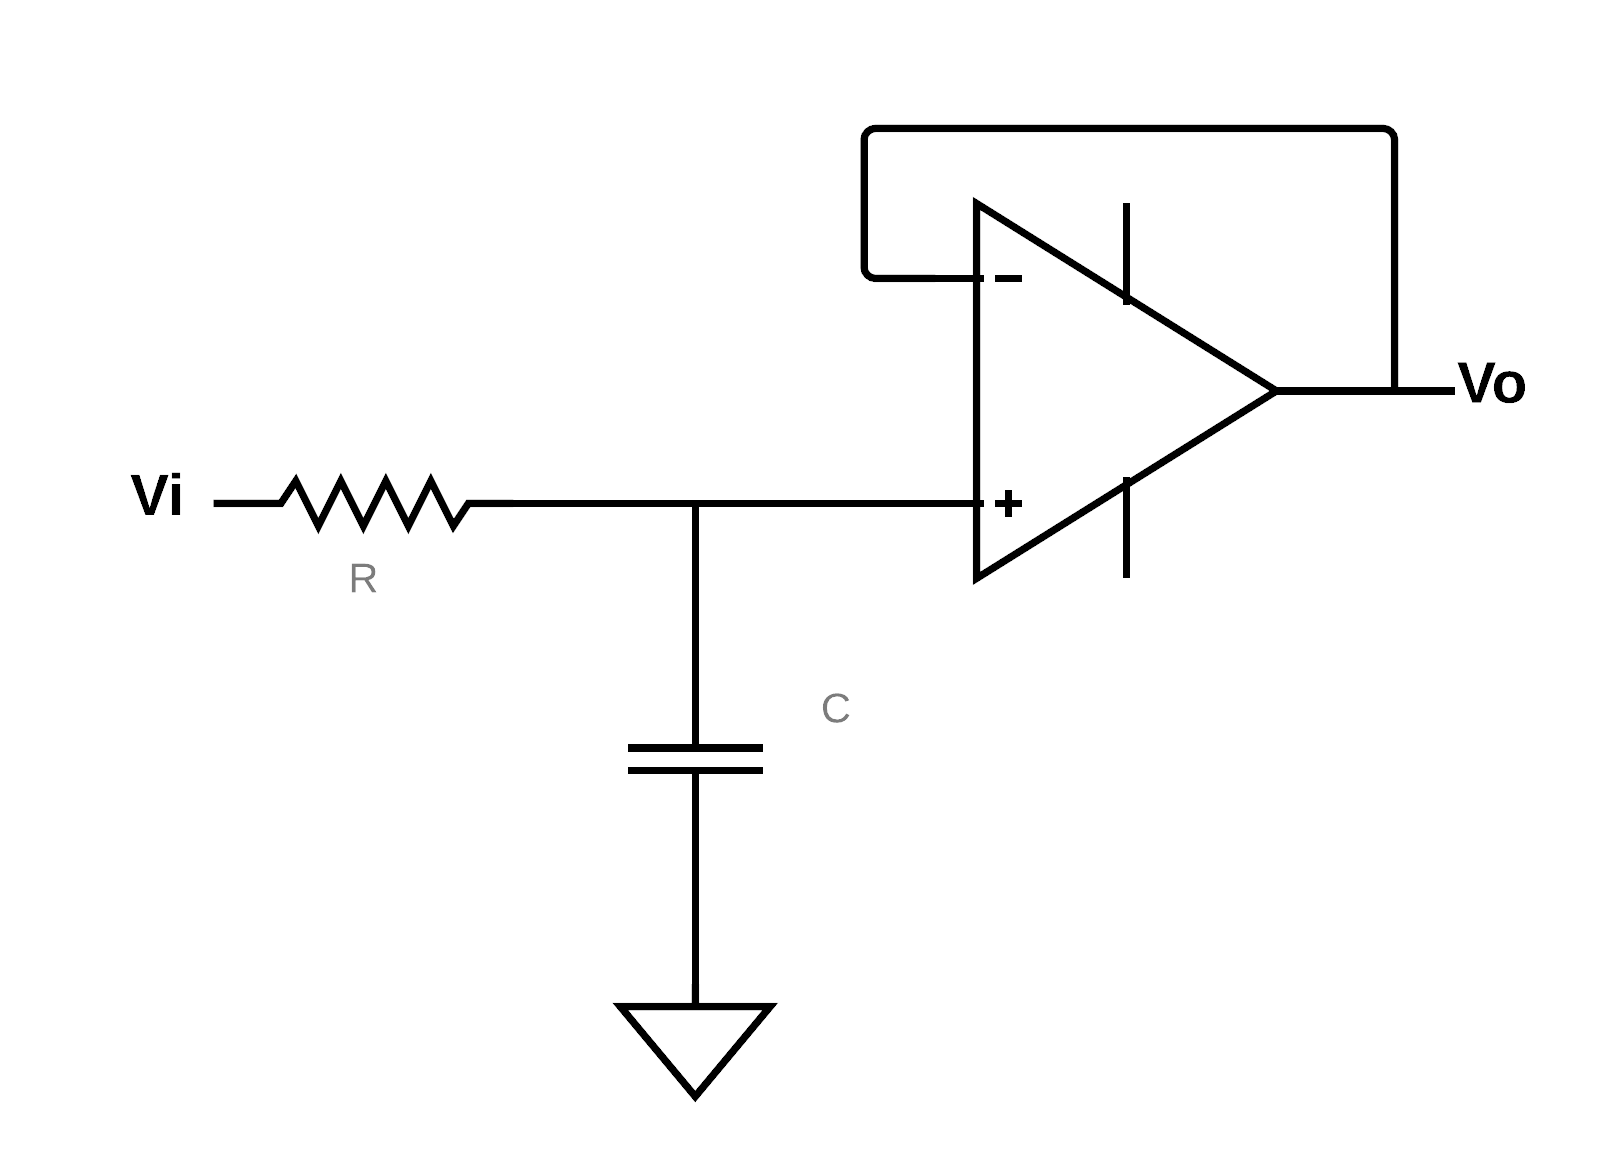
\includegraphics[width= 0.5\textwidth]{../Ejercicio2-DisenoDeCeldas/1CeldaSallenKey/images/LowPassRC.png}
    \caption{Circuito Low Pass primer orden.}
    \label{fig:1LPGain}
\end{figure}

Analizando el circuito de la figura \ref{fig:1LPGain} se plantea rápidamente el siguiente sistema. Se considera $A_{Vol}$ constante y $Z_{IN_{OpAmp}}\rightarrow \infty$, de modo que la corriente hacia el amplificador operacional resulta nula. Se obtiene su función transferencia e impedancia de entrada.

\begin{equation}
\left\{\begin{matrix}
        I_{in} = \frac{V^{+}-0}{\frac{1}{sC}}
        \\
        I_{in} = \frac{V_{in} - V^{+} }{R}
        \\
        V_{o} = V^{-}
        \\
        V_{o}=A_{Vol} (V^{+} - V^{-})
\end{matrix}\right.
    \label{eq:SK5}
\end{equation}


\begin{equation}
        H(s) = \frac{A_{Vol}}{(A_{Vol}+1)(sCR + 1)} \approx \frac{1}{sCR + 1}
    \label{eq:SK6}
\end{equation}

\begin{equation}
        Z_{in} = R + \frac{1}{sC} 
    \label{eq:SK7}
\end{equation}

Donde si $s = j0 \Rightarrow Z_{in} \rightarrow  \infty$, la impedancia de entrada ideal de un amplificador operacional, y con $s = j0 \rightarrow \infty \Rightarrow Z_{in} = R$

Otra opción para implementar esta etapa sería el \textbf{integrador inversor compensado}, el cual permite incrementar la atenuación en banda pasante del filtro. No obstante, a los fines de la transferencia solicitada, basta con utilizar el circuito descripto arriba, el cual a su vez no invierte la fase. 

\subsection{Celda de segundo orden Sallen Key: Análisis}

La figura \ref{fig:SK_H} muestra la configuración pasa-bajos de la celda Sallen Key. Para su análisis se consideró nuevamente $A_{Vol}$ constante y $Z_{IN_{OpAmp}}\rightarrow \infty$. A partir de la relación de corrientes en el nodo $V_{1}$ se obtiene la función transferencia y la impedancia de entrada.

\begin{figure}[H]
    \centering
    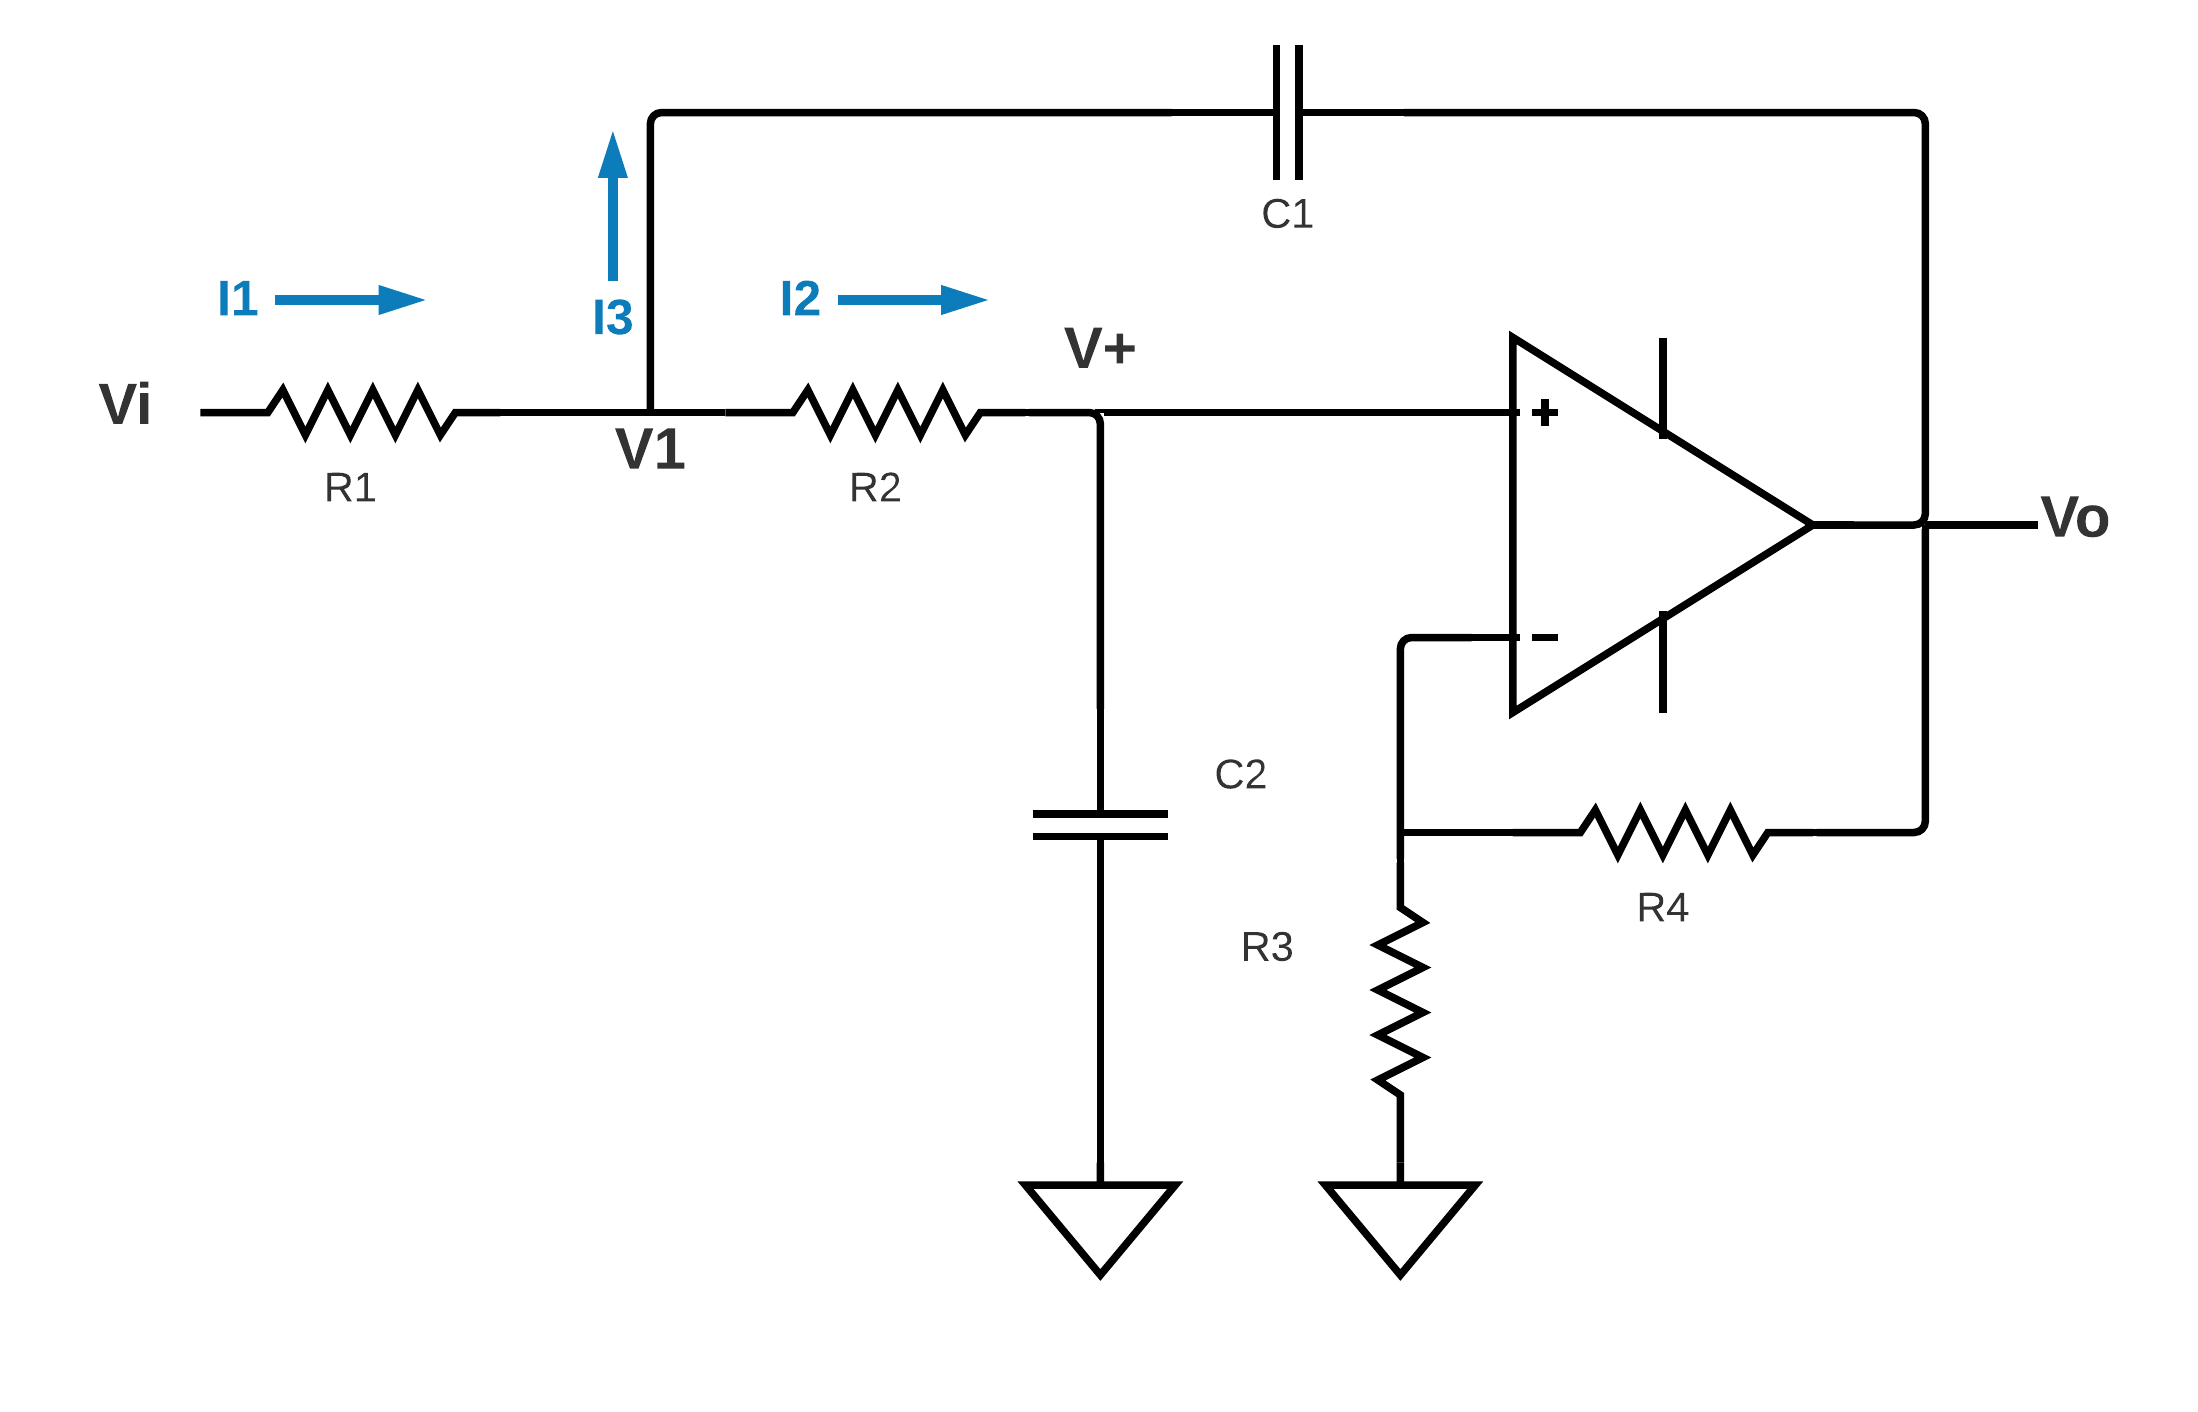
\includegraphics[width= 0.75\textwidth]{../Ejercicio2-DisenoDeCeldas/1CeldaSallenKey/images/SallenKeyH.png}
    \caption{Análisis de Sallen Key Low Pass}
    \label{fig:SK_H}
\end{figure}

\begin{equation}
\left\{\begin{matrix}
       V_{o} = A_{Vol} \cdot (V^{+}-V^{-})
        \\
        V^{-} = V_{o} \cdot \frac{R_{3}}{R_{3}+R_{4}} = V_{o} \cdot \frac{1}{K}
        \\
        V^{+} = V_{1} \cdot \frac{\frac{1}{sC_{2}}}{R_{2}+\frac{1}{sC_{2}}} = \frac{V_{1}}{sC_{2}R_{2} + 1}
        \\
        \frac{V_{i}-V_{1}}{R_{1}} - \frac{V_{1}-0}{R_{2}+\frac{1}{sC_{2}}} - \frac{V_{1}-V_{o}}{\frac{1}{sC_{1}}} = 0
\end{matrix}\right.
    \label{eq:SK8}
\end{equation}

\begin{equation}
    H(s)=\frac{A_{Vol}\cdot K}{(A_{Vol}+K)\cdot(s^{2}\cdot R_{1}C_{1}R_{2}C_{2} + s\cdot \frac{A_{Vol}((R_{2}+R_{1})C_{2}+R_{1}C_{1}(1-K))+K(R_{1}C_{1}+(R_{2}+R_{1})C_{2})}{A_{Vol}+K} + 1)}
    \label{eq:SK9}
\end{equation}

Para la cual:


$$ w_{0} = \frac{1}{\sqrt{R_{1}C_{1}R_{2}C_{2}}} $$


$$Q = \frac{(A_{Vol}+K)\sqrt{R_{1}C_{1}R_{2}C_{2}}}{A_{Vol}((R_{2}+R_{1})C_{2}+R_{1}C_{1}(1-K))+K(R_{1}C_{1}+(R_{2}+R_{1})C_{2})} $$

$$G = \frac{A_{Vol}(R_{3} + R_{4})}{A_{Vol}R_{3} + R_{3} + R_{4}}$$

$$K = \frac{R_{3}+R_{4}}{R_{3}}$$

Empleando el caso mas ideal, para el que $A_{Vol} \rightarrow \infty$, se obtiene la siguiente función transferencia:

\begin{equation}
    H(s) = \frac{K}{\frac{s^{2}}{(\frac{1}{\sqrt{R_{1}C_{1}R_{2}C_{2}}})^{2}} + s\cdot [R_{1}C_{1}(1-K)+(R_{2}+R_{1})C_{2}] + 1} 
    \label{eq:SK11}
\end{equation}

$$w_{0} = \frac{1}{\sqrt{R_{1}C_{1}R_{2}C_{2}}}$$

$$Q = \frac{\sqrt{R_{1}C_{1}R_{2}C_{2}}}{R_{1}C_{1}(1-K)+(R_{2}+R_{1})C_{2}}$$

Teniendo que la impedancia de entrada se define como $Z_{in} = \frac{V_{in}}{I_{1}}$, a partir del mismo sistema \ref{eq:SK8} resulta:


\begin{equation}
Z_{in} = \frac{C_{1}C_{2}R_{1}R_{2}(A_{Vol} + K)s^{2} + (A_{Vol}C_{1}R_{1}(1-K) + A_{Vol}C_{2}(R_{1} + R_{2}) + K(C_{1}R_{1} + C_{2}R_{1} + C_{2}R_{2}))s + A_{Vol} + K}{(C_{1}C_{2}R_{2}(A_{Vol} + K))s^{2} + s(A_{Vol}C_{1}(1-K) + K(C_{1} + C_{2}) + A_{Vol}C_{2})}
    \label{eq:SK11}
\end{equation}

En el caso mas ideal con $A_{Vol} \rightarrow \infty$, la impedancia de entrada obtiene la siguiente expresión:

\begin{equation}
Z_{in}(s)=\frac{s^{2}\cdot C_{1}C_{2}R_{1}R_{2} + s \cdot (C_{2}R_{1} + C_{2}R_{2} + C_{1}R_{1} (1-K)) + 1}{s^{2}\cdot C_{1}C_{2}R_{2} + s\cdot (C_{2} + C_{1}(1-K))}
    \label{eq:SK12}
\end{equation}

\subsection{Sensibilidades}

La sensibilidad relativa de una función y respecto a una variable x está dada por $S^{y}_{x} = \frac{x}{y}\frac{\partial y}{\partial x}$. Se analizan las sensibilidades para el factor de calidad Q, la frecuencia de corte $w_{0}$ y la ganancia G considerando $A_{Vol}$ constante. Recordando que $K = \frac{R_{3}+R_{4}}{R_{3}}$ es la ganancia ideal de la celda, se calculan las sensibilidades respecto a las variables involucradas en cada uno. 

$$Q = \frac{(A_{Vol}+K)\sqrt{R_{1}C_{1}R_{2}C_{2}}}{A_{Vol}((R_{2}+R_{1})C_{2}+R_{1}C_{1}(1-K))+K(R_{1}C_{1}+(R_{2}+R_{1})C_{2})} $$

\begin{table}[H]
\centering
\begin{tabular}{c|c}
x         & $S^{Q}_{x}$                                                                                                                                             \\ \hline
\\
$R_{1}$   & $\frac{1}{2} - \frac{QR_{1}((R_{2}+R_{1})C_{2}+R_{1}C_{1}(1-K))}{(A_{Vol}+K)\sqrt{R_{1}C_{1}R_{2}C_{2}}}$           
\\
\\
$R_{2}$   & $\frac{1}{2} - \frac{QR_{2}(A_{Vol}C_{2}+KC_{2}))}{(A_{Vol}+K)\sqrt{R_{1}C_{1}R_{2}C_{2}}}$                                                  
\\
\\
$R_{3}$   & $\frac{A_{Vol}+1}{A_{Vol}+K} - \frac{Q(A_{Vol}(R_{2}+R_{1})C_{2}+R_{1}C_{1}+(R_{2}+R_{1})C_{2})}{(A_{Vol}+K)\sqrt{R_{1}C_{1}R_{2}C_{2}}}$
\\
\\
$R_{4}$   & $\frac{R_{4}}{A_{Vol}R_{3}+R_{3}+R_{4}} - \frac{QR_{4}((R_{2}+R_{1})C_{2}+R_{1}C_{1}-A_{Vol}R_{1}C_{1})}{(A_{Vol}R_{3}+R_{3}+R_{4})\sqrt{R_{1}C_{1}R_{2}C_{2}}}$
\\
\\
$C_{1}$   & $\frac{1}{2} - \frac{QC_{1}((KR_{1})+A_{Vol}R_{1}(1-K))}{(A_{Vol}+K)\sqrt{R_{1}C_{1}R_{2}C_{2}}}$
\\
\\
$C_{2}$   & $\frac{1}{2} - \frac{QC_{2}(A_{Vol}(R_{2}+R_{1})+K(R_{2}+R_{1})))}{(A_{Vol}+K)\sqrt{R_{1}C_{1}R_{2}C_{2}}}$
\\
\\
$A_{Vol}$ & $\frac{A_{Vol}}{A_{Vol}+K}\left [ 1 - \frac{Q((R_{2}+R_{1})C_{2}+R_{1}C_{1}(1-K))}{(A_{Vol}+K)\sqrt{R_{1}C_{1}R_{2}C_{2}}} \right ]$
\\
\\
K         & $\frac{K}{A_{Vol}+K} - \frac{QK((R_{2}+R_{1})C_{2}+R_{1}C_{1}-A_{Vol}R_{1}C_{1})}{(A_{Vol}+K)\sqrt{R_{1}C_{1}R_{2}C_{2}}}$  
\\
\end{tabular}
    \label{table:SQ}
\end{table}

$$ w_{0} = \frac{1}{\sqrt{R_{1}C_{1}R_{2}C_{2}}} $$

\begin{table}[H]
\centering
\begin{tabular}{c|c}
x       & $S^{w_{0}}_{x}$ \\ \hline
\\
$R_{1}$ & $-\frac{1}{2}$
\\
\\
$R_{2}$ & $-\frac{1}{2}$
\\
\\
$C_{1}$ & $-\frac{1}{2}$
\\
\\
$C_{2}$ & $-\frac{1}{2}$
\\
\end{tabular}
\label{table:SW}
\end{table}

$$G = \frac{A_{Vol}(R_{3} + R_{4})}{A_{Vol}R_{3} + R_{3} + R_{4}}$$

\begin{table}[H]
\centering
\begin{tabular}{c|c}
x         & $S^{G}_{x}$                                                                 \\ \hline
\\
$A_{Vol}$ & $1 - \frac{1}{K}$                                                           \\
\\
$R_{3}$   & $\frac{R_{3}}{R_{3}+R_{4}} - \frac{R_{3}(A_{Vol}+1)}{A_{Vol}(R_{3}+R_{4})}$ \\
\\
$R_{4}$   & $\frac{R_{4}}{R_{3}+R_{4}} - \frac{R_{4}(A_{Vol}+1)}{A_{Vol}(R_{3}+R_{4})}$
\\
\end{tabular}
\label{table:SG}
\end{table}

Resulta de interés recalcar que a medida que $A_{Vol} \rightarrow \infty$, la sensibilidad de Q respecto a $A_{Vol}$ tiende a cero, lo esperado en el caso mas ideal. 

\subsection{Diseño de filtro}


Se procederá a diseñar las etapas del filtro pasa-bajos solicitado mediante las celdas analizadas. Para facilidad del diseño, se aproximará $A_{Vol}$ A infinito a modo de emplear las ecuaciones transferencias mas ideales. Ambas etapas cuentan con $w_{0} = w_{p} = 20 \pi 3300 Hz = 20734.5 \frac{rad}{s}$. 

Para la implementación de la celda se decidió emplear los amplificadores operacionales del integrado TL084, el cual presenta buenos parámetros de ganancia, GBP y alto slew rate. Para los resistores, se considerarán los valores de las series E24 y E96 de 1\% de tolerancia. Se emplearán capacitores cerámicos multicapa de 10 \% tolerancia. 


\textbf{Primera etapa: filtro pasa-bajos orden uno con seguidor de tensión.} Planteando la expresión de la frecuencia de corte, se puede obtener la relación entre R y C. En esta etapa, se busca cumplir con la condición de impedancia de entrada del filtro $Z_{in}$ mayor igual que $50k \Omega$; se verá luego que la impedancia de entrada del filtro se mantiene por encima de ese valor para todo el rango de frecuencias analizada. Debido que los valores de capacitores son menos abundantes, se plantea un capacitor de $470 pF$. Con esto, se calcula la resistencia de la primera etapa:

$$w_{0} = \frac{1}{RC}$$

Proponiendo $C = 470pF \Rightarrow R = 102616,9 \Omega \approx 102k \Omega + 1k \Omega$ Preset.

Por lo tanto, se plantea implementar la primera etapa con un capacitor $C = 470 pf$ y $R = 102000 \Omega$ + Preset $1k\Omega$ para ajuste fino. 


\textbf{Segunda etapa: celda Sallen Key pasa-bajos.} Para implementar la celda Sallen Key estudiada es conveniente adoptar un criterio de diseño, tanto para facilitar el calculo de los componentes como para imponer condiciones. Se busca asegurar el cumplimiento de Q = 1 y K = 1. Una forma óptima de encarar el diseño es plantear el diseño con ganancia unitaria y componentes proporcionales. De este modo, se tiene que:

\begin{equation}
\begin{matrix}
R_{1} = mR_{2} = mR & ; & C_{2} = nC_{2} = nC
\end{matrix}
    \label{eq:SK13}
\end{equation}

\begin{equation}
\begin{matrix}
w_{0} = \frac{1}{\sqrt{mn}RC} & ; & Q = \frac{\sqrt{mn}}{1+m} \Rightarrow  1 + 2m + m^{2} = \frac{mn}{Q^{2}}
\end{matrix}
    \label{eq:SK14}
\end{equation}

Imponiendo la condición que $m > 0$:

\begin{equation}
\begin{matrix}
m = \frac{n}{Q^{2}} - 1 + \sqrt{(\frac{n}{Q^{2}} - 1)^{2} - 1} & ; & m > 4Q^{2}
\end{matrix}
    \label{eq:SK14}
\end{equation}

Intentando asegurar esta ultima condición entre m y Q y asegurando Q = 1, se plantearon distintos valores de C a modo de cumplir la relación para luego calcular los valores de n, R2 y R1. Se iteró este procedimiento hasta obtener valores convenientes y cercanos a los normalizados de las series E24 o E96. Finalmente, se impuso que $C_{2} = C = 4.7nF$ y $C_{1} = 22nF$.se tiene que $n = 4.681$ y $m = 2.232$. De este modo, se obtienen $R_{2} = 3175 \Omega$ y $R_{1} = 7086 \Omega$. Normalizando a valores de la serie E96:

$$R_{2} = 3160 \Omega$$
$$R_{1} = 6980 \Omega + Preset 500 \Omega$$

Para lograr K = 1, se conecta directamente la entrada inversora del OpAmp con su salida. Lo cual otorga una frecuencia de corte idealmente de w0 = tanto y Q = 1.0019. 



\subsection{Respuesta en frecuencia y análisis Monte Carlo}

Con los valores de los componentes fijados, se realizaron simulaciones en LTspice para observar el comportamiento en frecuencia del filtro y comparar la respuesta obtenida con respecto a la función transferencia teórica con los componentes normalizados y a la aproximación calculada por Butterworth. Se decidió realizar la simulación considerando las resistencias implementadas con presets con los valores resultantes de los calculos y no directamente los normalizados. 

\begin{figure}[H]
    \centering
    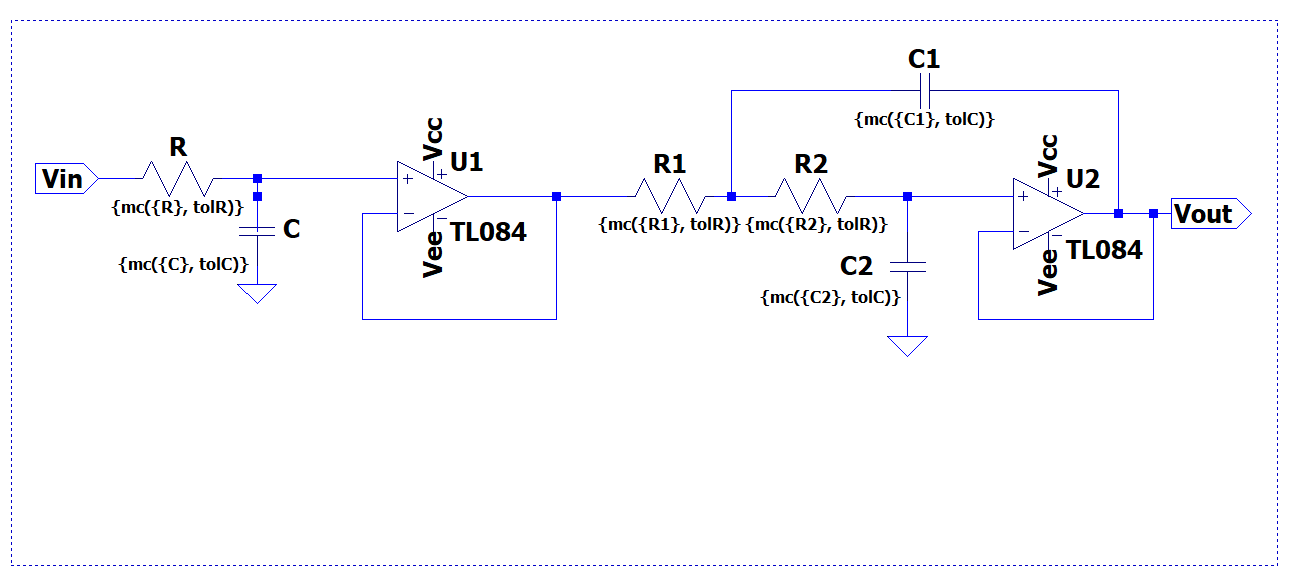
\includegraphics[width= 0.7\textwidth]{../Ejercicio2-DisenoDeCeldas/1CeldaSallenKey/images/circLTspiceSK.png}
    \caption{Circuito simulado en LTspice.}
    \label{fig:simuSK}
\end{figure}

\begin{figure}[H]
    \centering
    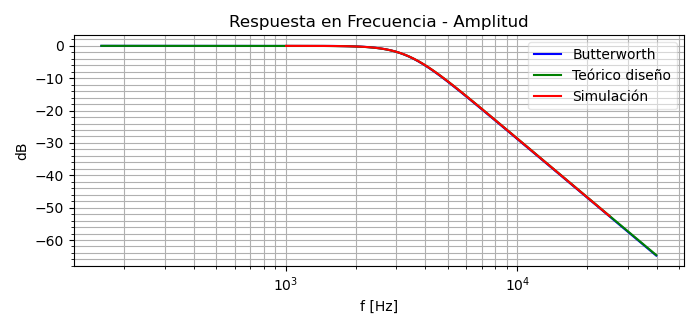
\includegraphics[width= 0.7\textwidth]{../Ejercicio2-DisenoDeCeldas/1CeldaSallenKey/images/SKGain.png}
    \caption{Respuesta en frecuencia de filtro implementado con resistores serie E96 sin ajuste de preset: Ganancia}
    \label{fig:SKGain}
\end{figure}

\begin{figure}[H]
    \centering
    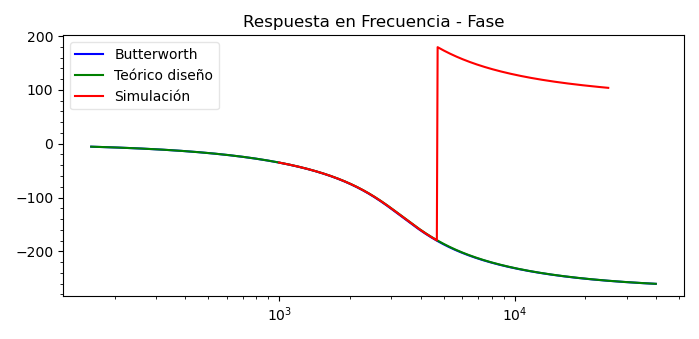
\includegraphics[width= 0.7\textwidth]{../Ejercicio2-DisenoDeCeldas/1CeldaSallenKey/images/SKphase.png}
    \caption{Respuesta en frecuencia de filtro implementado con resistores serie E96 sin ajuste de preset: diferencia de fase}
    \label{fig:SKphase}
\end{figure}

Se observa en la figura \ref{fig:SKGain} que las ganancias de las transferencias obtenidas por la aproximación de Butterworth, la implementada en el diseño del filtro y la simulación coinciden en gran medida para el rango de frecuencia de transición de banda de paso a banda atenuada. Por lo tanto, el filtro implementado cumple la plantilla. El salto en la fase en la simulación frente a los teóricos se puede deber a que la función implementada en el $Plot Tool$ toma la fase en otro intervalo respecto a la simulada. Desde la simulación, como se verá seguidamente, se observa que desde el panel de simulación la fase continúa descendiendo mas allá de los -180\circ.

Para estudiar el impacto de la tolerancia de los componentes en la respuesta en frecuencia, se realizó un análisis Monte Carlo. Como se mencionó anteriormente, se emplearon resistores con tolerancia de 1\% y capacitores con tolerancia del 10\%. Para el análisis se fijaron los componentes a los valores comerciales. Primeramente se observó el impacto de las variaciones de los componentes en el comportamiento del filtro en su totalidad y luego se vio el caso individual de cada celda. 

\begin{figure}[H]
    \centering
    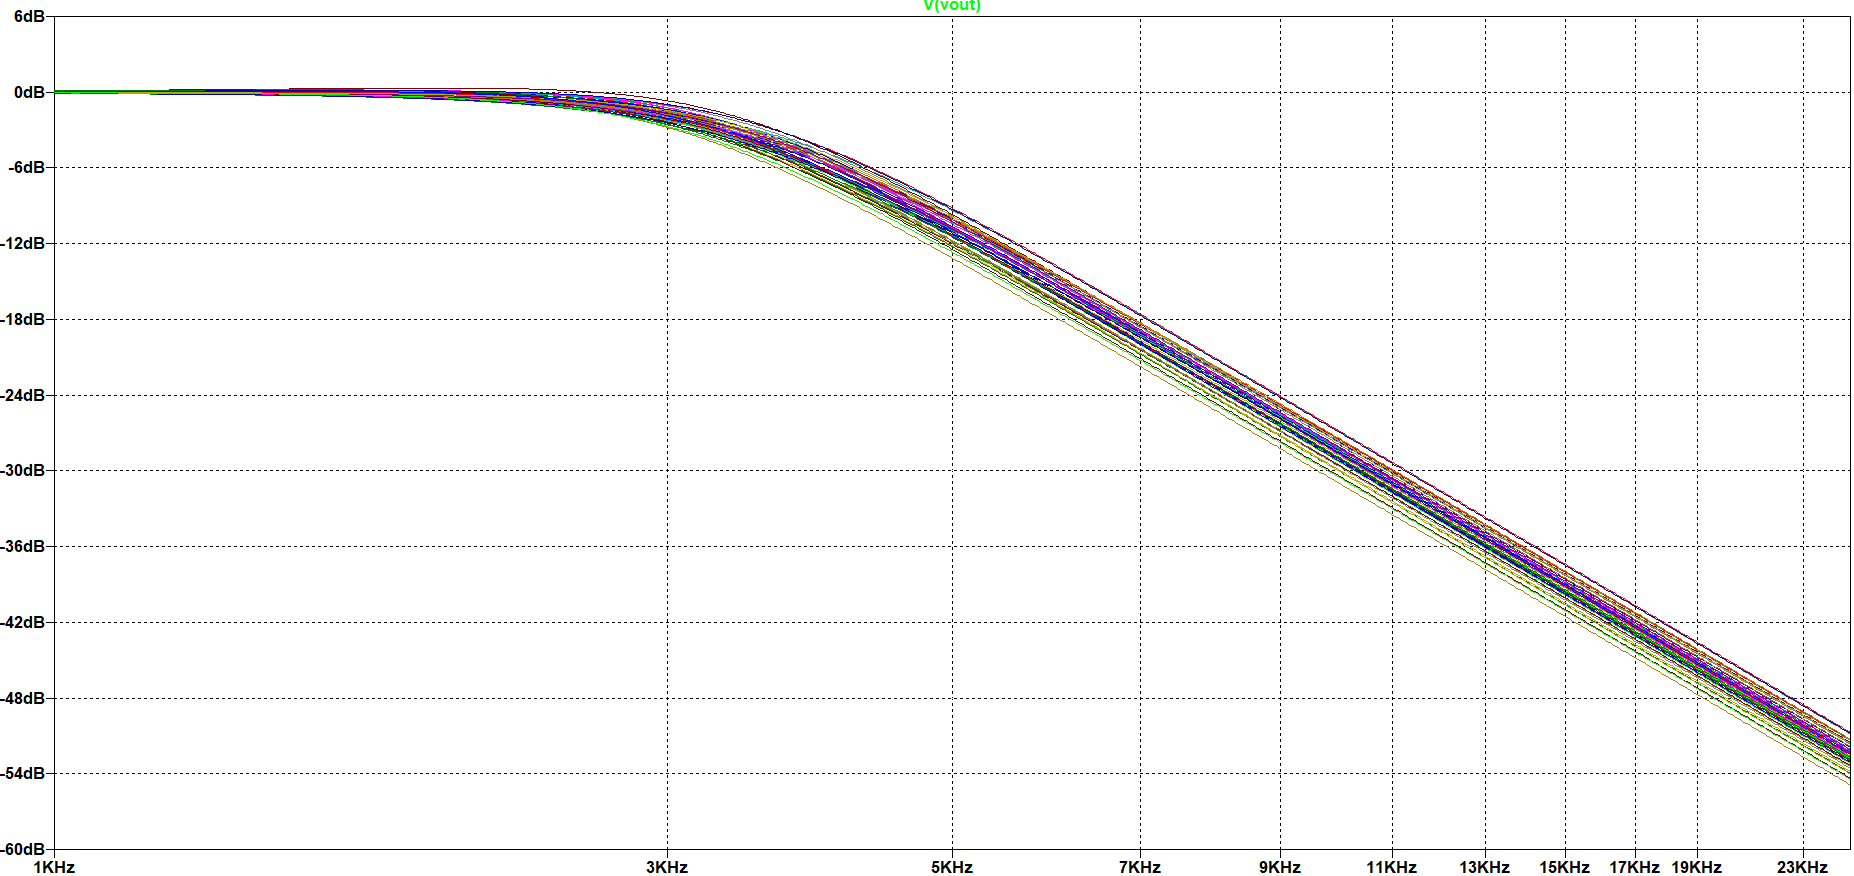
\includegraphics[width= 0.7\textwidth]{../Ejercicio2-DisenoDeCeldas/1CeldaSallenKey/images/simuMagNormalizados.png}
    \caption{Simulación respuesta en frecuencia con tolerancias: Ganancia.}
    \label{fig:simugain}
\end{figure}

\begin{figure}[H]
    \centering
    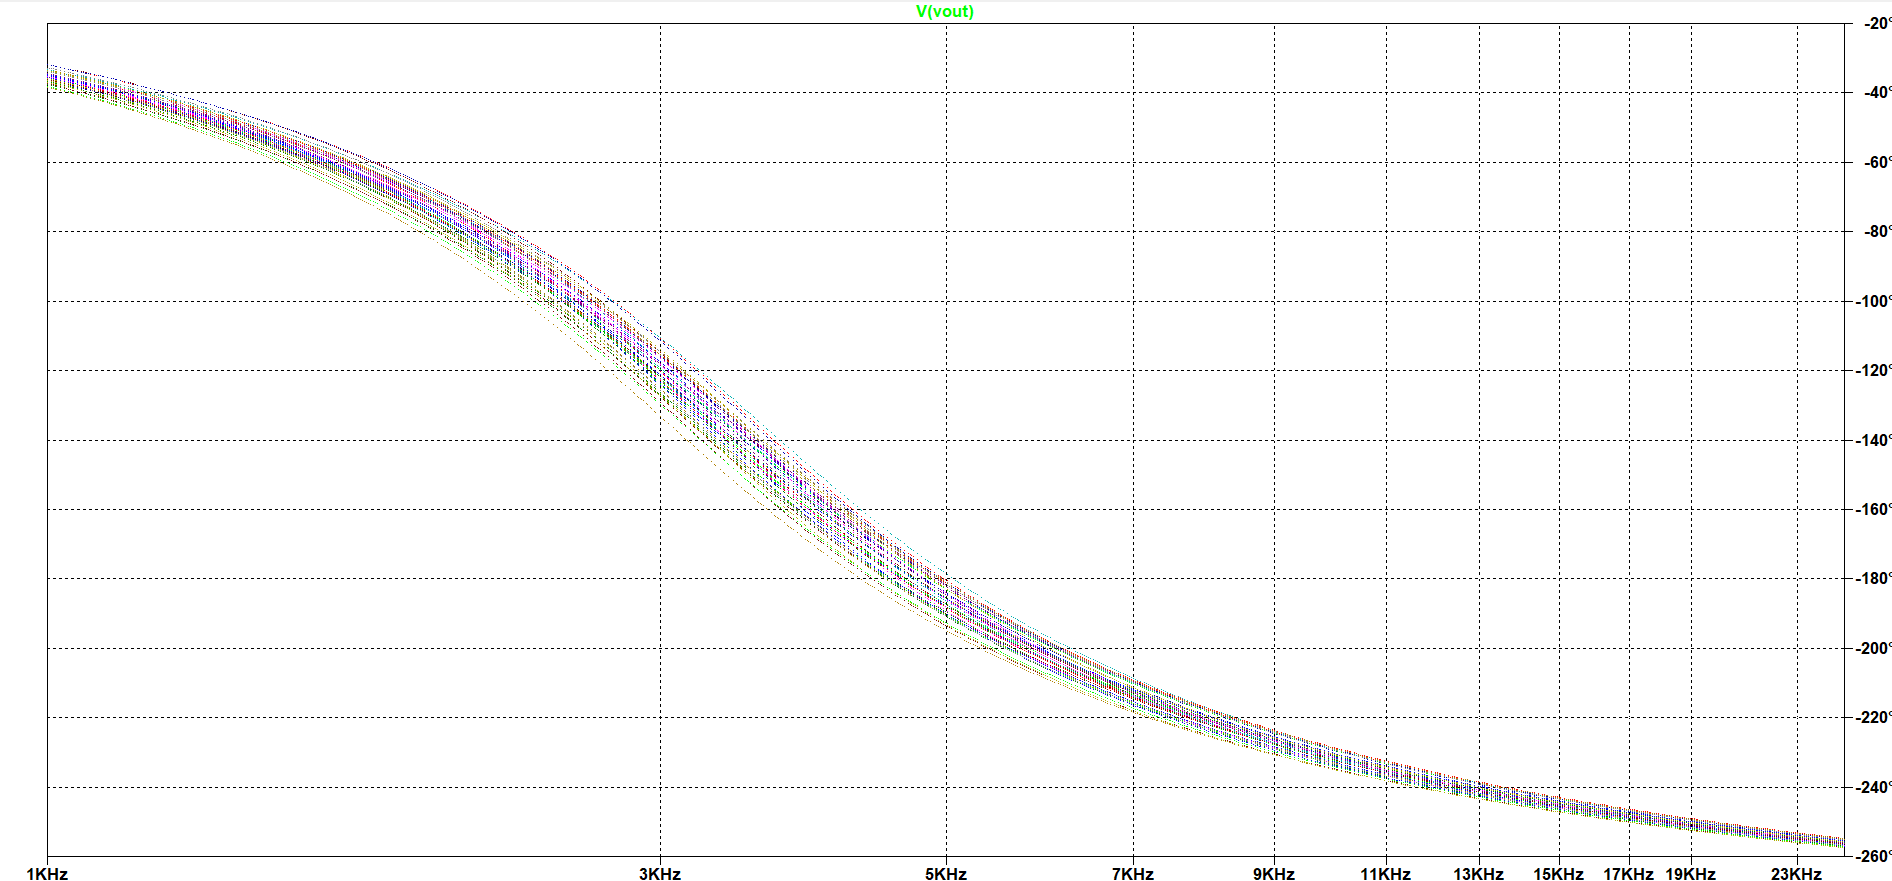
\includegraphics[width= 0.7\textwidth]{../Ejercicio2-DisenoDeCeldas/1CeldaSallenKey/images/simuFaseNormalizados.png}
    \caption{Simulación respuesta en frecuencia con tolerancias: Ganancia.}
    \label{fig:simuphase}
\end{figure}

\begin{figure}[H]
    \centering
    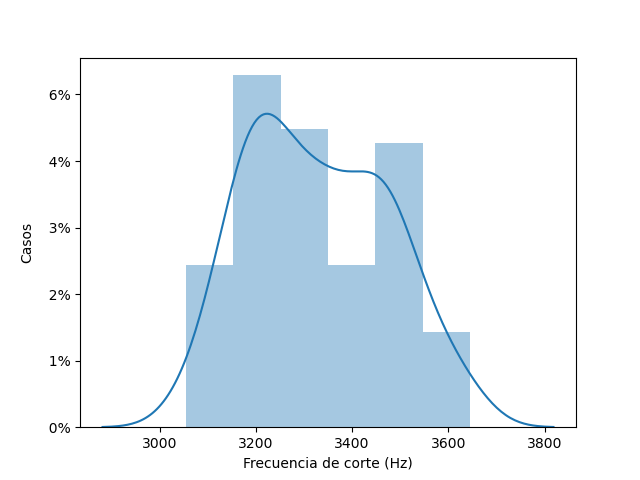
\includegraphics[width= 0.7\textwidth]{../Ejercicio2-DisenoDeCeldas/1CeldaSallenKey/images/MCSinPreset.png}
    \caption{Histograma análisis Monte Carlo con resistores serie E96.}
    \label{fig:MCE96}
\end{figure}

\begin{figure}[H]
    \centering
    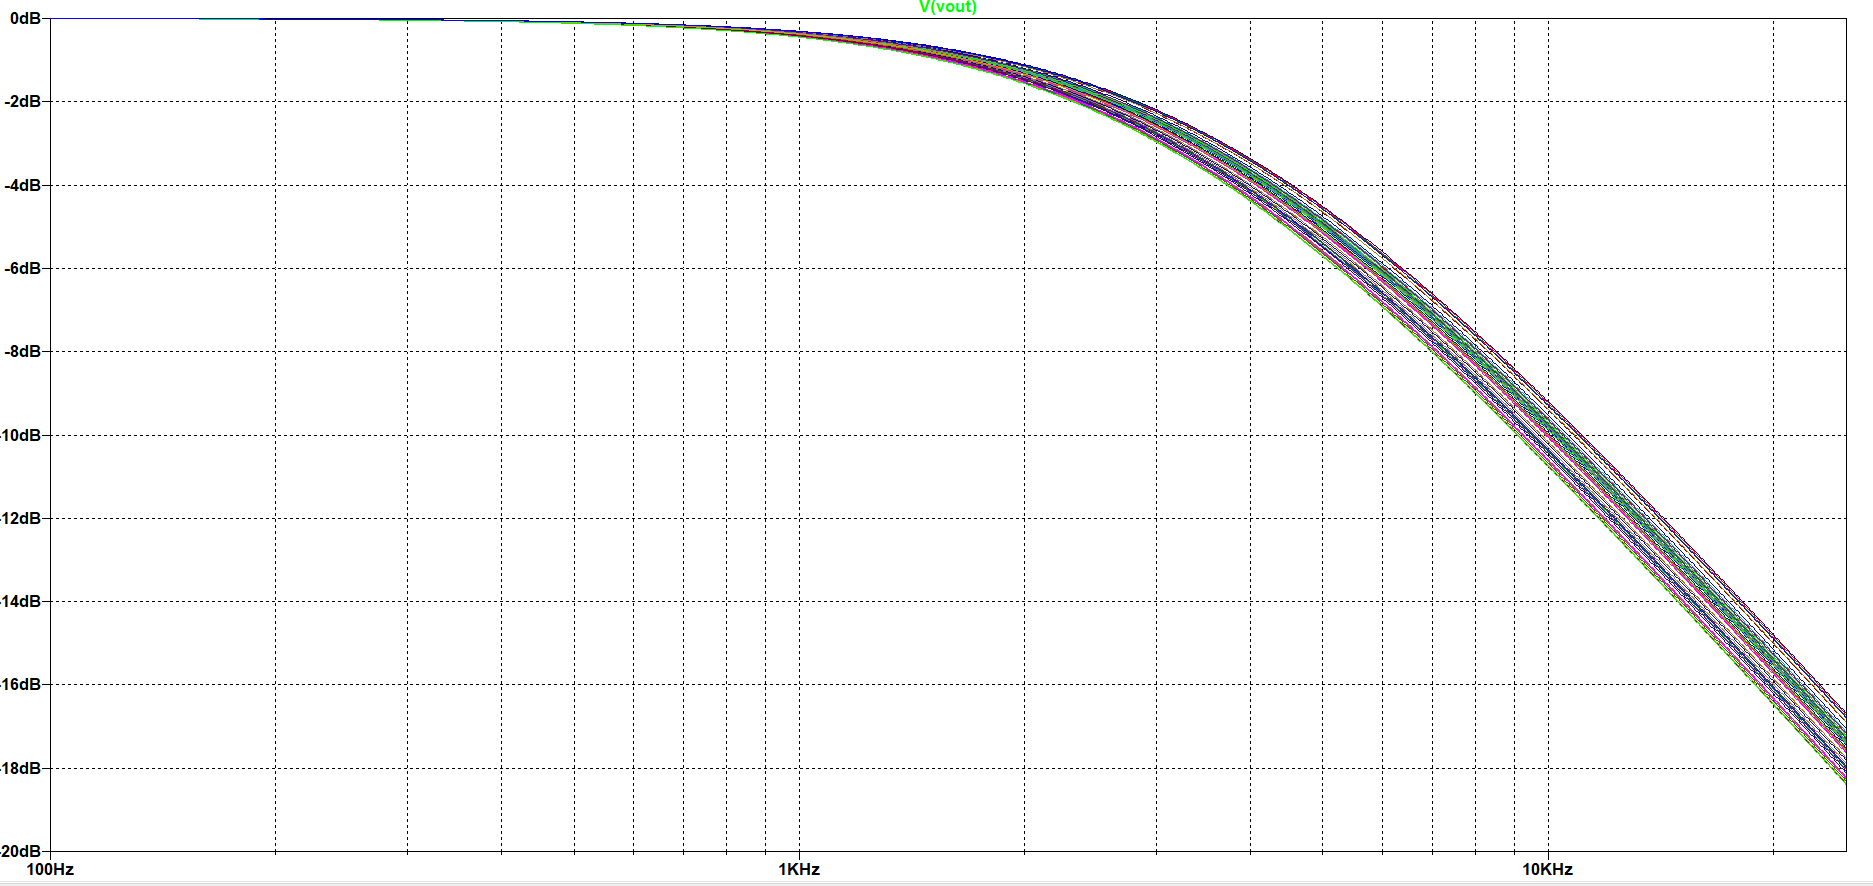
\includegraphics[width= 0.7\textwidth]{../Ejercicio2-DisenoDeCeldas/1CeldaSallenKey/images/MAG1stOrder.png}
    \caption{Celda primer orden. Simulación de respuesta en frecuencia con tolerancias: Ganancia.}
    \label{fig:1LPsimugain}
\end{figure}

\begin{figure}[H]
    \centering
        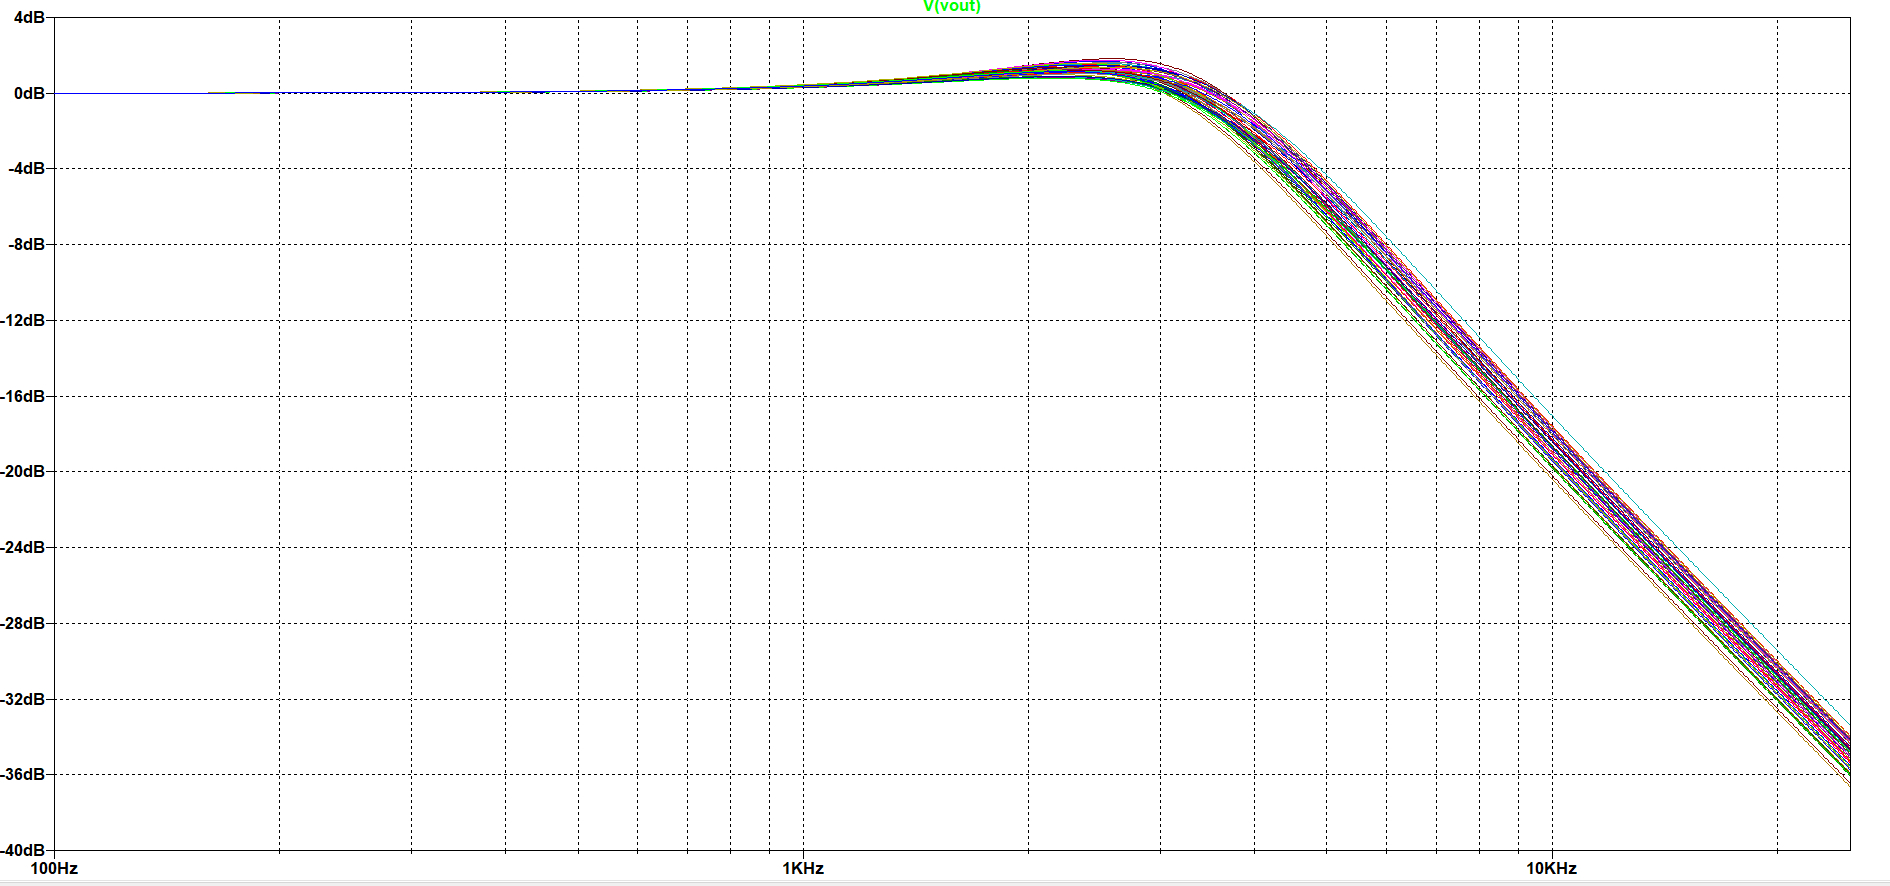
\includegraphics[width= 0.7\textwidth]{../Ejercicio2-DisenoDeCeldas/1CeldaSallenKey/images/SKsimu.png}
    \caption{Celda Sallen Key. Simulación de respuesta en frecuencia con tolerancias: Ganancia.}
    \label{fig:SKsimugain}
\end{figure}

Con el histograma del filtro \ref{fig:MCE96} se puede observar que la mayoría de las curvas pasan a $-3dB$ alrededor de la frecuencia de corte planteada de 3.3KHz. Sin embargo, un aspecto importante de la plantilla solicitada es que a esa frecuencia se buscaba una atenuación como máximo de $-3dB$. Para cumplir con esa condición, es deseable que la mayoría de las curvas sufran esa atenuación para una frecuencia igual o mayor que la $f_{p} = 3300Hz$. Por ello, se analizó la opción de implementar el filtro con valores de resistencias menores y correspondientes a la serie E24, ya que son valores normalizados mas comunes para construir luego el filtro. Con esto en mente, se plantea implementar $R=100k\Omega$ + preset $25k\Omega$, $R_{2}3k\Omega$ y $R_{1}=6,8kOmega$ + preset $500\Omega$. Simulando con estos valores, se observó el corrimiento de las curvas a frecuencias un poco mayores. Asimismo, se obtendría una $Q = 0.9970$ para la celda Sallen Key, por lo que no se afectaría el comportamiento buscado. Por otro lado, puede ser conveniente ser mas conservadores en cuanto a plantear primeramente una frecuencia de corte mayor, ya que con los presets en serie a R y a $R_{1}$ se puede "correr" la frecuencia de corte a valores menores. 

\begin{figure}[H]
    \centering
    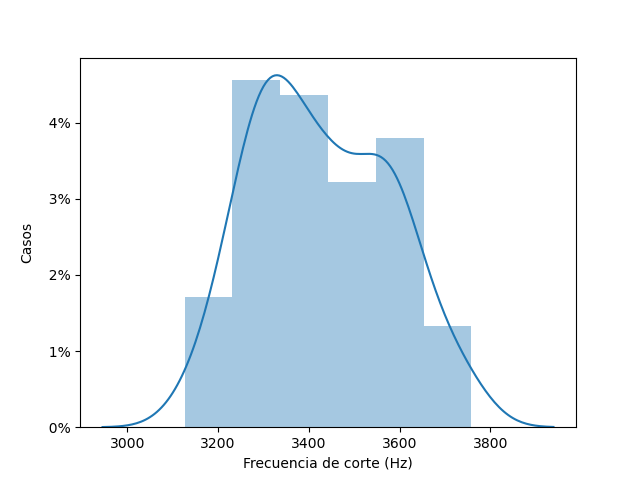
\includegraphics[width= 0.7\textwidth]{../Ejercicio2-DisenoDeCeldas/1CeldaSallenKey/images/MCE24.png}
    \caption{Histograma análisis Monte Carlo con resistores serie E24.}
    \label{fig:MCE96}
\end{figure}

Asimismo, se simuló la magnitud de la impedancia de entrada. Se observa que esta se mantiene siempre por encima de los $50k\Omega$. 

\begin{figure}[H]
    \centering
        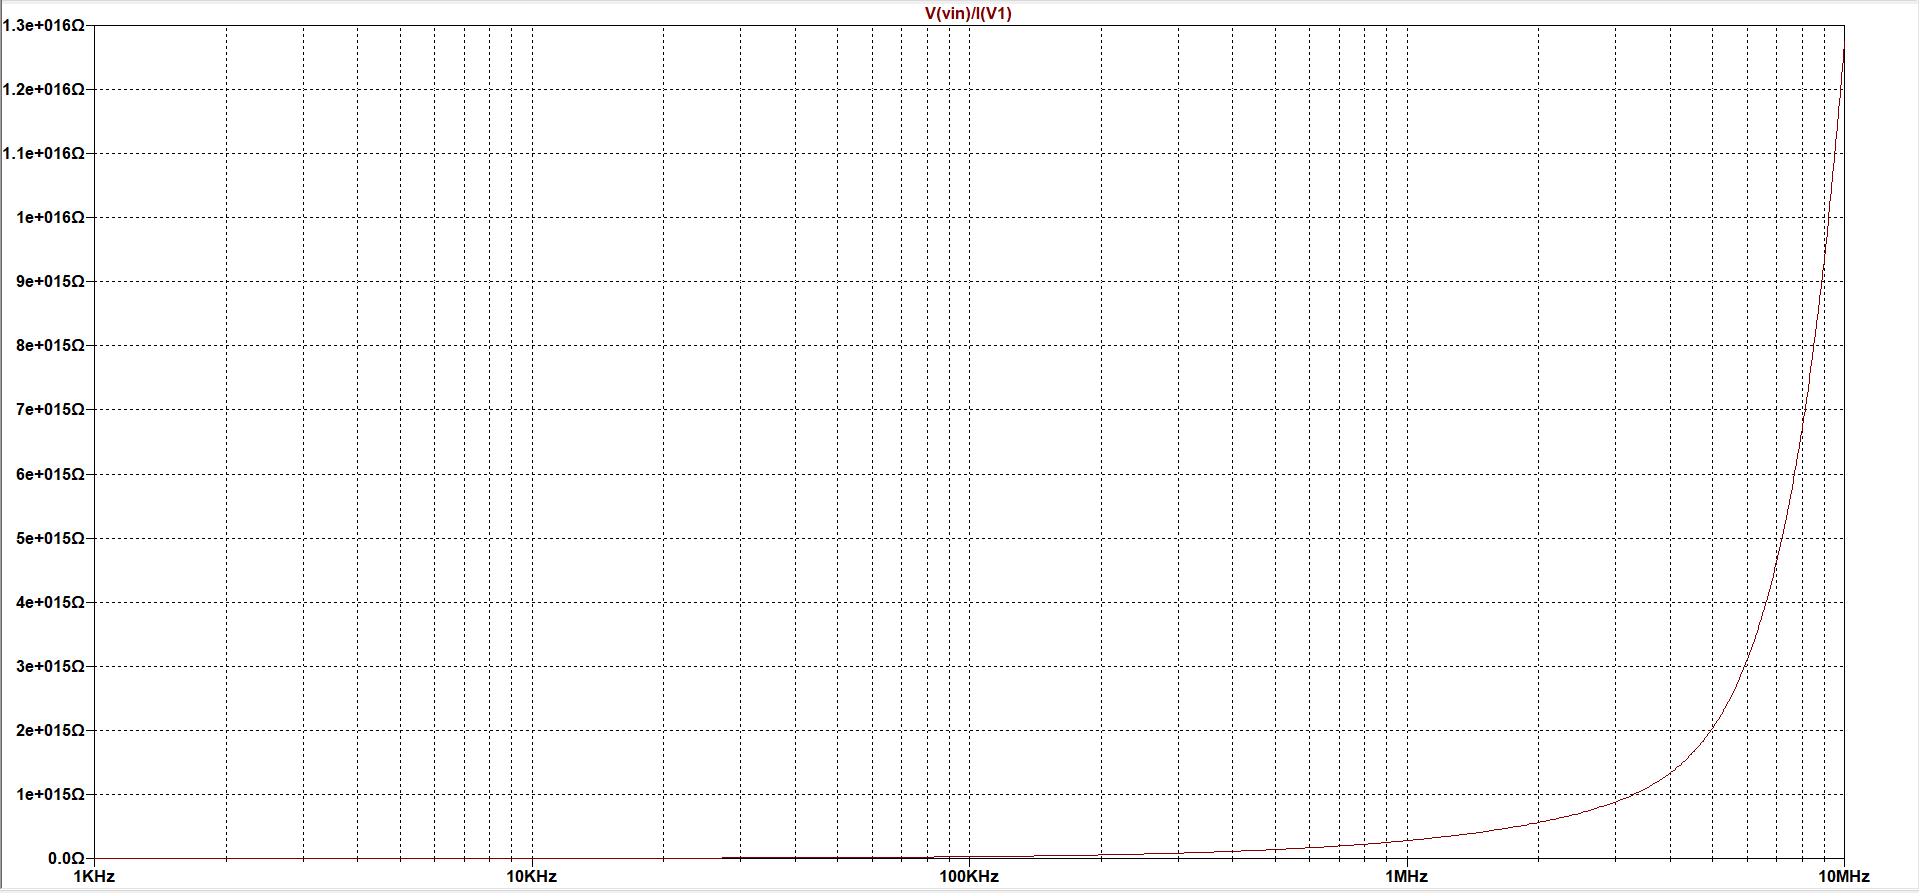
\includegraphics[width= 0.7\textwidth]{../Ejercicio2-DisenoDeCeldas/1CeldaSallenKey/images/Zin.png}
    \caption{Respuesta en frecuencia de magnitud de impedancia de entrada.}
    \label{fig:Zin}
\end{figure}



En cualquier caso, será necesario calibrar el filtro para cumplir con la plantilla. Emplea los resistores propuestos por último mueven en mayor medida la frecuencia a valores mayores al deseado, pero mediante los presets implementados en cada etapa puede regularse. Para esto, se propone verificar si la frecuencia a la que se da una atenuación de $-3dB$ supera los $3300Hz$; siendo ese el caso, se debe pasar a ajustar el valor de la resistencia $R$ en el filtro pasa bajos de primer orden. Para un ajuste fino de la $f_{p}$ y la Q, se puede regular el preset asociado a la $R_{1}$.



\subsection{Restricciones por ganancia y factor de calidad}

Si bien la celda Sallen Key resulta versátil para implementar un filtro de segundo orden, presenta restricciones en cuanto a factor de calidad Q y ganancia K. En el circuito implementado en esta sección del informe, tanto la K como la Q de la Sallen Key fueron unitarias, por lo que no se visualizaron las restricciones. Sin embargo, a partir del análisis de sensibilidades se observa que la Q está relacionada con todas las variables del circuito, por lo que se puede ver muy afectado por sus variaciones. En particular, las restricciones se acentúan al momento del diseño. En el caso de imponer condición de componentes iguales, es decir $C_{2} = C_{1} = C$ y $R_{2} = R_{1} = R$, se tiene que la Q queda directamente relacionada con la ganancia con $Q = \frac{1}{3-K}$. Por lo tanto, se pierde independencia del diseño. Por las sensibilidades, este circuito no es recomendable para implementar filtros con $Q<5$. 

En cuanto a la ganancia, es posible agregar una derivación a la entrada con la cual se obtiene una transferencia con ganancia multiplicada por un factor "a".

\begin{figure}[H]
    \centering
        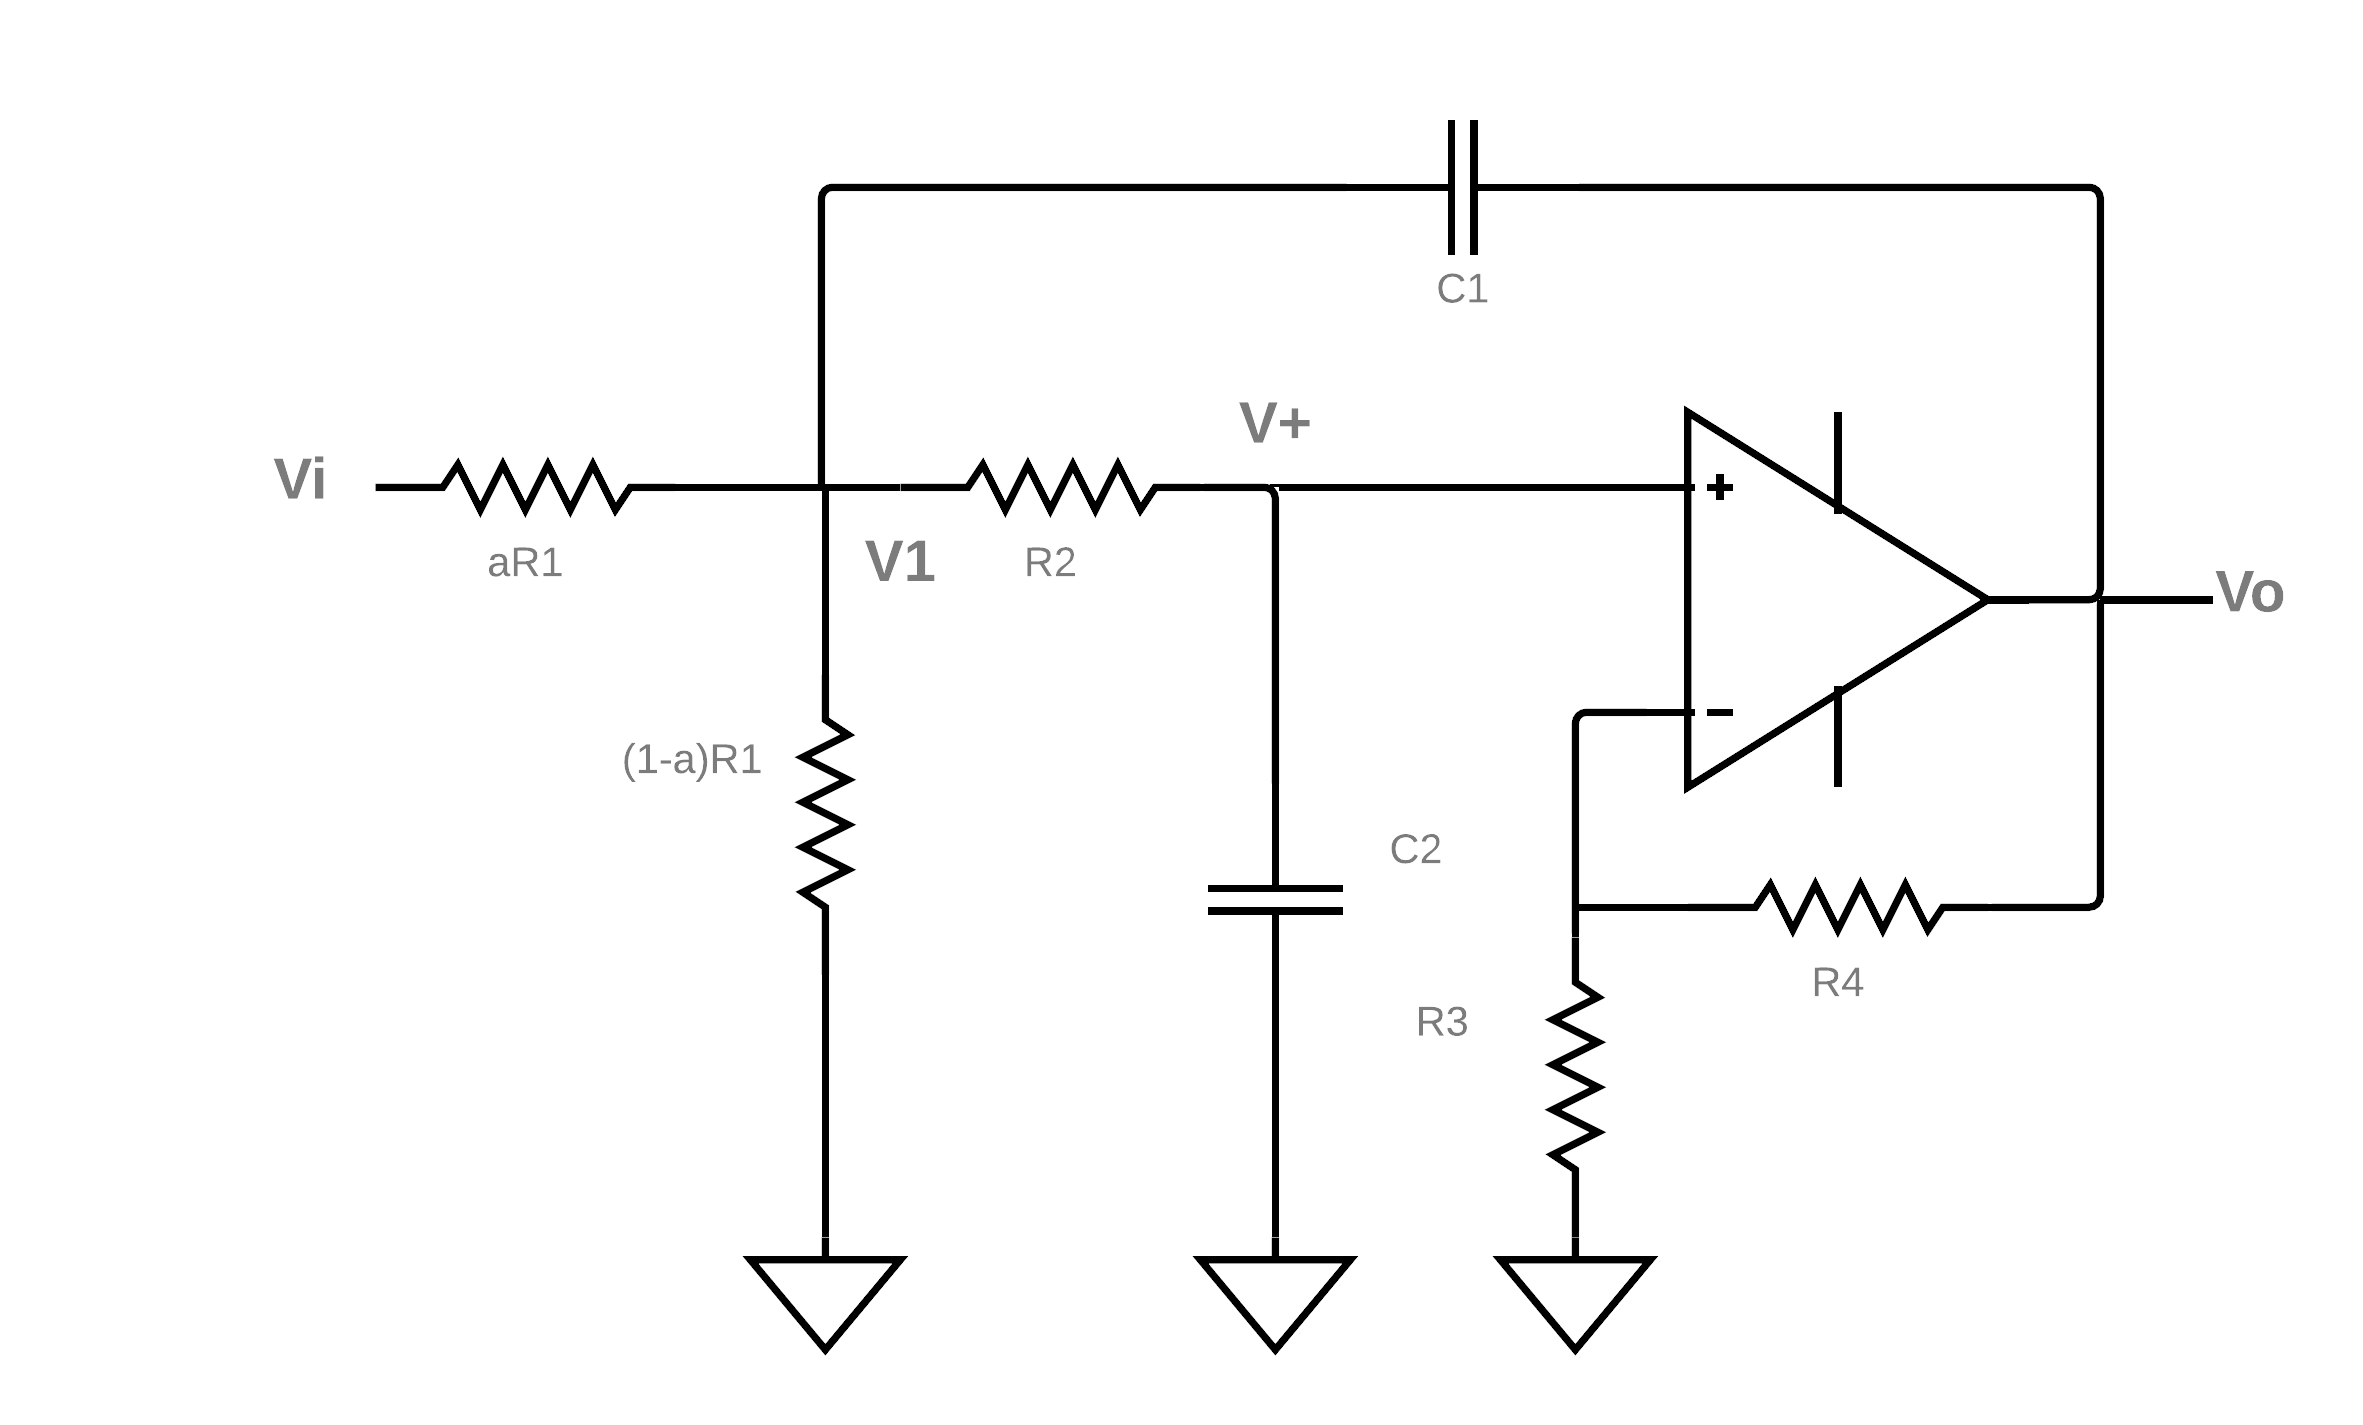
\includegraphics[width= 0.7\textwidth]{../Ejercicio2-DisenoDeCeldas/1CeldaSallenKey/images/SallenKeyGain.png}
    \caption{Celda Sallen Key con derivación de ganancia.}
    \label{fig:SKGain}
\end{figure}


\subsection{Conclusiones}

Se pudo observar que los resultados simulados se corroboraron de forma excelente respecto a las transferencias calculadas. En pocas palabras, la celda Sallen Key resultó óptima para implementar el filtro solicitado y cumplir con las características de la aproximación de Butterworth; se logra un comportamiento con máxima planicie en banda pasante y una caída monótona en banda atenuada. 

Por otro lado, la celda Sallen Key resulta de sencilla implementación ya que pueden adoptarse distintos criterios de diseño para calcular sus componentes. La adoptada en este informe se debió a las restricciones en ganancia y factor de calidad. Es importante recalcar que además las características solicitadas en la plantilla fueron ideales para emplear una celda Sallen Key ya que otorgaban valores bajos de Q y K. De haber sido mucho mayores alguno de ellos, no se hubiera podido conseguir el comportamiento deseado facilmente con este tipo de celda, siendo esa la principal desventaja que presenta. 


\section{Celda Rauch (Deliyannis-Friend modificada)}

\subsection{Introducción}

Se busca mediante el uso de una celda de Rauch o también conocida como Deliyannis-Friend y la aproximación de Chebyshev para diseñar un filtro pasa banda con las siguientes parámetros:

\begin{table}[H]
    \centering
    \resizebox{0.5\textwidth}{!}{%
    \begin{tabular}{cc}
    \hline
    \multicolumn{2}{c}{Par\'ametros de diseño} \\ \hline
    Pendiente de pasabajos normalizado & -40dB/dec \\
    $f_p$ & 64KHz \\
    B & 1/10 \\
    $A_p$ & 3dB \\
    $Z_{in}(f)$ & $\geq 50K\Omega$ \\
    Filtro & Pasa-Banda\\\hline
    \end{tabular}%
    }
    \caption{Par\'ametros de diseño para el filtro a implementar}
    \label{ej22diseno}
\end{table}

Para ello debemos primero introducir la celda de Rauch que tiene la forma:

\begin{figure}[H]
    \centering
    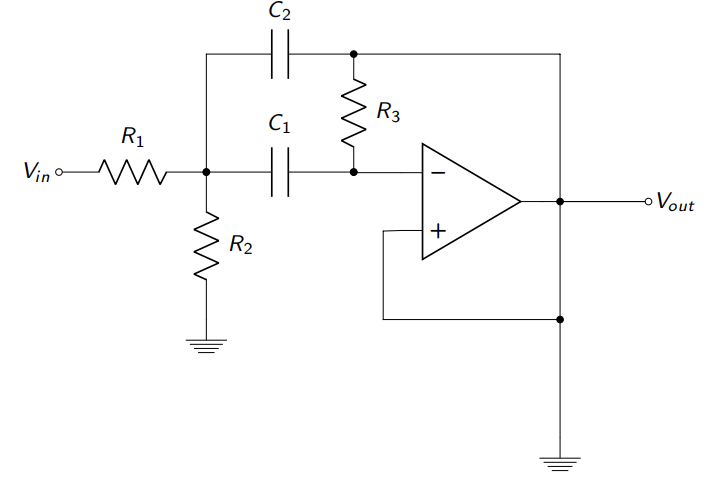
\includegraphics[scale = 0.6]{../Ejercicio2-DisenoDeCeldas/2CELDARAUCH/Informe/circuito3.png}
    \caption{Celda de Rauch}
    \label{ej22cirbasic}
\end{figure}

Sin embargo, se observa que uno de los requisitos que debe cumplir el filtro es que $B = \frac{1}{Q} = \frac{1}{10}$, un valor de Q hace que las relaciones entre las resistencias R1 y R2 sean muy elevados, puesto que los valores de estas resistencias son inversa y directamente proporcionales, respectivamente, a este valor. Es por ello que se utiliza la versión modificada de la la celda Deliyannis-Friend que hace uso de un ciclo de realimentación positiva logrando asi valores elevados de Q.

\begin{figure}[H]
    \centering
    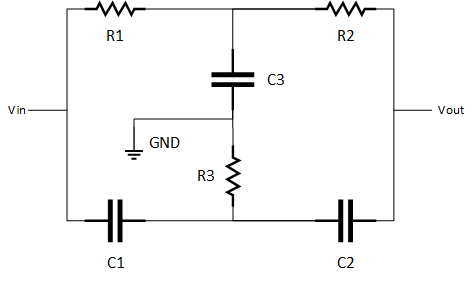
\includegraphics[scale = 0.6]{../Ejercicio2-DisenoDeCeldas/2CELDARAUCH/Informe/circuito.png}
    \caption{Celda de Rauch Mejorada}
    \label{ej22cirbasic}
\end{figure}

Luego analizando el circuito con amplificadores operacionales ideales, o sea los $A_{vol} \longrightarrow \infty$, nos queda que la transferencia de la misma es:
\begin{equation}
    \label{ej22eqh}
    H(s) = \frac{sC2R2R3(RA+RB)}{s^2(C1C2R1R2R3RB) + s(C1R1R2RB + C2(R1R2RB - RA(R1R3 + R2R3))) + RB(R1+R2)}
\end{equation}
Conociendo que las resistencia de retroalimentación valen $RA = KR$ y $RB = (1-K)R$ y si conciderando los capacitores iguales ($C = C1 = C2$) obtenemos que:
\begin{equation}
    \label{ej22eqq}
    Q = \frac{\sqrt{R1R2R3(R1 + R2)}}{2R1R2 - \frac{K}{1 -K} (R1 + R2)R3}
\end{equation}
\begin{equation}
    \label{ej22eqw0}
    \omega_0^2 = \frac{R1+R2}{C^2R1R2R3}
\end{equation}
\begin{equation}
    \label{ej22eqg}
    G = \frac{R2R3}{2R1R2(K - 1) + KR3(R1 + R2)}
\end{equation}

\subsection{Dise\~no del Filtro con Chebyshev}

Para obtener una funci\'on trasferencia que cumpla con una plantilla, es posible utilizar la aproximación\'on de Chebyshev cuyas f\'ormulas caracter\'isticas se muestran en \ref{ej22eqche}.
\begin{equation}
    \begin{split}
        |H(s)|^2 = \frac{1}{1+\epsilon^2 \cdot T_n^2(\omega_N)}, \hspace{0.2cm} \epsilon = \sqrt{10^{\frac{A_p}{10}}-1}
    \end{split}
    \label{ej22eqche}
\end{equation}
Donde $T_n(\omega)$ son los polinomios de Chebyshev.

Debido a que se pide una pendiente de pasa bajos normalizado de $40dB/dec$, el orden de dicho pasa bajos es $n=2$, luego desnormalizando la aproximación, se encuentra que el orden del filtro pasa-banda es 4. En consecuencia, se
utilizarán 2 celdas Rauch de orden 2. Además, se pide una atenuación máxima en banda pasante de $3dB $ pero debido a las tolerancias de los componentes es óptimo una $A_p = 1dB$ para tener margen de error.

Luego, sabiendo que es un filtro pasa-banda podemos establecer la siguiente relación:
\begin{equation}
    \begin{split}
        f_0^2=f_P^+ \cdot f_P^-\\
        B=\frac{\Delta f}{f_0}\\
    \end{split}
    \label{ej22eqb}
\end{equation}

En resumen el filtro tendrá las siguientes propiedades:

\begin{table}[H]
    \centering
    \resizebox{0.4\textwidth}{!}{%
    \begin{tabular}{cc}
    \hline
    \multicolumn{2}{c}{Parámetros de diseño} \\ \hline
    Orden normalizado [n] & 2 \\
    Orden del filtro & 4 \\
    $f_p^+$ & 67kHz \\
    $f_p^-$ & 61kHz \\
    $A_p$ & 1dB \\ \hline
    \end{tabular}%
    }
    \caption{Propiedades del Filtro a Dise\~nar}
    \label{tab:TEMPLATE}
\end{table}

Teniendo en cuenta dichas propiedades, la transferencia del circuito sera:
\begin{equation}
\begin{split}
    H(s) &= \frac{s^2 B^2 \omega_0^2}{s^4+s^3 B \omega_0 1.0977343  + s^2 \omega_0^2 (2+B^2 1.1025103) + s B \omega_0^31.0977343 + \omega_0^4}\\
     &= \frac{ 1.62 \cdot 10^9 s^2}{s^4+ 44.14 \cdot 10^3  s^3 +  3.25 \cdot 10^{11} s^2+  7.13 \cdot 10^{15} s+ 2.61 \cdot10^{22}}
\end{split}
\end{equation}

Como se menciono, utilizaremos dos celdas Rauch en cascada por lo que podemos diseñar el circuito separando la transferencia en dos etapas factorizando, resultando en:
\begin{equation}
    \label{ej22eqhf}
    H(s) = 1.62 \cdot 10^9\frac{s}{s^2 + 21.01\cdot 10^3 s + 1.47 \cdot 10^{11}}\frac{s}{s^2 + 23.13\cdot 10^3 s+ 1.77 \cdot 10^{11}}
\end{equation}

Por otro lado para asegurar que la impedancia de entrada nunca sea menor a $50k\Omega$, se utilizaron 4 amplificadores operacionales. Dos de ellas para el funcionamiento de las celdas, uno se coloco como un buffer entre las dos etapas, asegurando que no se altere ninguna etapa, y el cuarto fue utilizado como buffer de entrada, es decir impedancias muy altas a las frecuencias de interés.


\subsection{Selección de Componentes}

Conociendo entonces la función de transferencia del circuito dado en la ecuación \ref{ej22eqhf} es posible determinar los componentes indicados para el filtro deseado. Estos componentes lo podemos determinar utilizando las siguientes relaciones dado por Schaumann con $Q_0 = 1.5$, el factor óptimo de calidad de la celda Deliyannis-Friend sin mejora, y las respectivas $Q$ y $\omega_0$ del las etapas:

\begin{equation}
\begin{split}
    &Q = \frac{Q_0}{1-2\alpha Q_0^2} \hspace{1.5CM} \alpha = \frac{K}{1-K}\\
    &H_B = \frac{HQ}{Q_0(1-K)} \hspace{1CM}
    R3 = \frac{2Q_0}{\omega_0 C}\\
    &R' = \frac{R3}{4Q_0^2} \hspace{2.3CM}
    a = \frac{H}{2Q_0^2}\\
    &R1 = \frac{R'}{a} \hspace{2.3CM}
    R2 = \frac{R'}{1-a}
\end{split}
\label{ej22eqvalor}
\end{equation}

Despejando desde las ecuaciones \ref{ej22eqvalor} con $C = 1nF$ obtenemos los componentes a utilizar idealmente.

% Please add the following required packages to your document preamble:
% \usepackage{booktabs}
\begin{table}[H]
\centering
\begin{tabular}{@{}ccc@{}}
\toprule
\textbf{Componente}                     & \textbf{Primera Etapa} & \textbf{Segunda Etapa} \\ \midrule
\textbf{C {[}$nF${]}}                     & 1                      & 1                      \\
\textbf{R1 ${[}\Omega{]}$} & 30.11k                 & 27.63k                 \\
\textbf{R2 ${[}\Omega{]}$} & 895.25                 & 815.69                 \\
\textbf{R3 ${[}\Omega{]}$} & 7.82k                  & 7.13k                  \\
\textbf{RA ${[}\Omega{]}$} & 2.03k                  & 2.03k                  \\
\textbf{RB ${[}\Omega{]}$} & 9.97k                  & 9.97k                  \\ \bottomrule
\end{tabular}
\caption{Componentes Ideales}
\label{ej22tvalt}
\end{table}

\subsubsection{Sensibilidad de los Componentes}

Es importante conocer las sensibilidades de los parámetros previo a la selección de componentes, de esta manera tener una idea de que valores pueden variar sin causar grandes cambios en el circuito. 


% Please add the following required packages to your document preamble:
% \usepackage{booktabs}
\begin{table}[H]
\centering
\begin{tabular}{@{}cccc@{}}
\toprule
\textbf{Componentes} & $S_x^w$     & $S_x^H $                                    & $S_x^Q$                                                     \\ \midrule
\textbf{C}           & $-\frac{1}{2}$           & $-\frac{(K-1)R1R2+KR3(R1+R2) }{2R1R2(K-1)+KR3(R1+R2)}$   & $\frac{KR3(R1+R2)}{2(((K-1)2R2+KR3)R1+KR2R3)  }                       $\\
\textbf{R1}          & $-\frac{ R2 }{ 2(R1+R2)}$ & $-\frac{R1(2R2(K-1)+KR3)}{ 2R1R2(K-1)+KR3(R1+R2)}    $    & $-\frac{R2((2R1(K-1)-KR3)R2-KR1R3)}{2(R1+R2)((2R1(K-1)+KR3)R2+KR1R3)} $   \\
\textbf{R2}          & $-\frac{ R1}{2(R1+R2)} $ & $\frac{KR1R3 }{(2R2(K-1)+KR3)R1+KR2R3}  $                 &$-\frac{R1(((K-1)2R2-KR3)R1-KR2R3)}{2(R1+R2)(((K-1)2R2+KR3)R1+KR2R3)}   $ \\
\textbf{R3}          & $-\frac{1}{2}$            &$\frac{2R1R2(K-1)}{(2R2(K-1)+KR3)R1+KR2R3}$               &$\frac{R1((K-1)2R2-KR3)-KR2R3}{2(R1((K-1)2R2+KR3)+KR2R3) }  $            \\
\textbf{K}           &$0 $                &$-\frac{2KR1R2+KR3(R1+R2)}{2R1R2(K-1)+KR3(R1+R2)} $       & $\frac{KR3(R1+R2)}{ (K-1)(R1((K-1)2R2+KR3)+KR2R3)}                 $   \\ \bottomrule
\end{tabular}
\label{ej22tst}
\caption{Ecuaciones de Sensibilidad}
\end{table}

\subsubsection{Selección de Componentes a Utilizar}

Como los valores no suelen ser comerciales se debe adaptar los valores, luego teniendo en cuenta sus sensibilidades se selecciono los componentes a implementar como:

% Please add the following required packages to your document preamble:
% \usepackage{booktabs}
\begin{table}[H]
\centering
\begin{tabular}{@{}ccccc@{}}
\toprule
\textbf{Componente}                     & \textbf{Primera Etapa} & \textbf{Implementación} & \textbf{Segunda Etapa} & \textbf{Implementación} \\ \midrule
\textbf{C {[}nF{]}}                     & 1                      & 1                       & 1                      & 1                       \\
\textbf{R1 ${[}\Omega{]}$} & 30.11k                 & 27k+3k                  & 27.63k                 & 27k+560                 \\
\textbf{R2 ${[}\Omega{]}$} & 895.25                 & 560+330                 & 815.69                 & 560+150+100             \\
\textbf{R3 ${[}\Omega{]}$} & 7.82k                  & 4.7k+3k+100             & 7.13k                  & 6.2k+1k                 \\
\textbf{RA ${[}\Omega{]}$} & 2.03k                  & 2k                      & 2.03k                  & 2k                      \\
\textbf{RB ${[}\Omega{]}$} & 9.97k                  & 10k                     & 9.97k                  & 10k                     \\ \bottomrule
\end{tabular}
\label{ej22tvalr}
\caption{Valores de Componentes Seleccionados}
\end{table}

Luego, realizando un análisis de montecarlo con los componentes utilizados, resistencia de tolerancia $5\%$ y capacitor de tolerancia $20\%$, se obtuvo los posibles casos que enfrentaríamos en una medición experimental.

\begin{figure}[H]
    \centering
    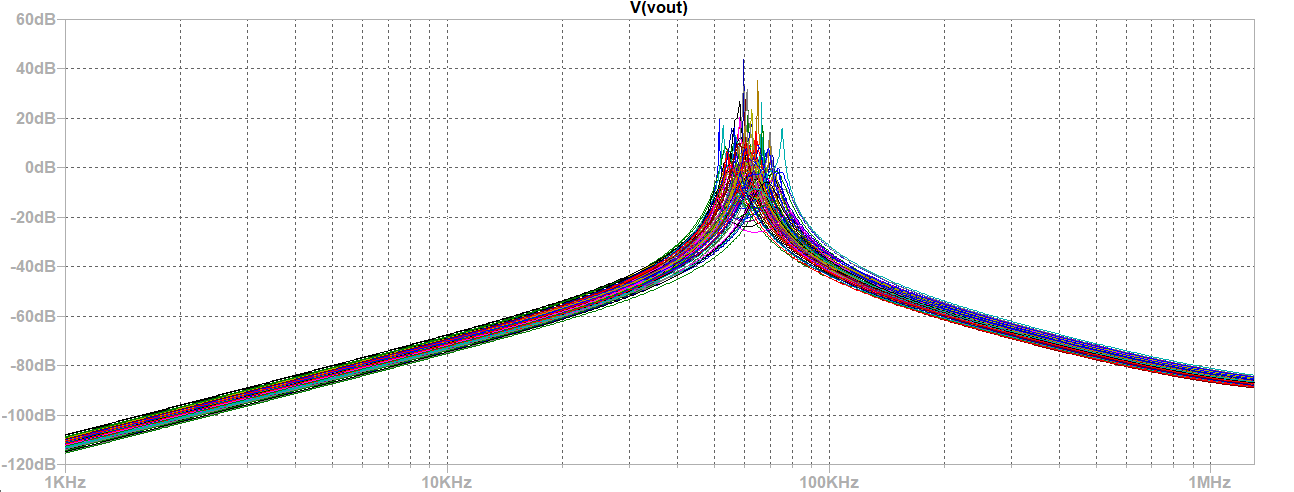
\includegraphics[scale = 0.65]{../Ejercicio2-DisenoDeCeldas/2CELDARAUCH/Informe/monte.PNG}
    \caption{Análisis de Montecarlo}
    \label{ej22monteall}
\end{figure}

Para una representación mas gráfica se realizo un histograma de dispersión por etapa para la verificar del correcto uso de los componentes.

\begin{figure}[H]
    \centering
    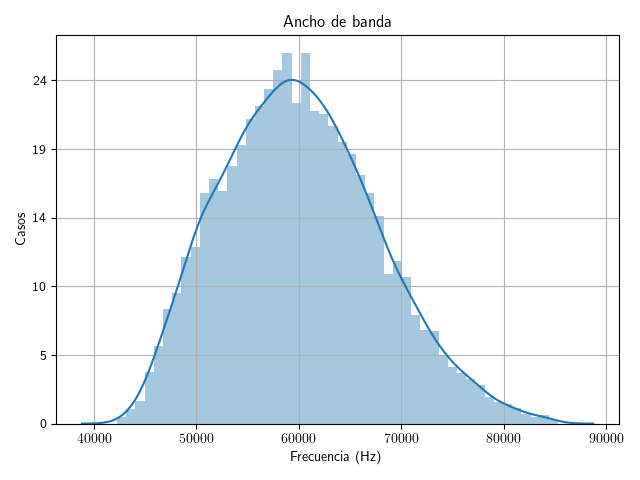
\includegraphics[scale = 0.5]{../Ejercicio2-DisenoDeCeldas/2CELDARAUCH/Informe/disp1.png}
    \caption{Histograma de Dispersión de f0 de la Primera Etapa}
    \label{ej22dis1}
\end{figure}

\begin{figure}[H]
    \centering
    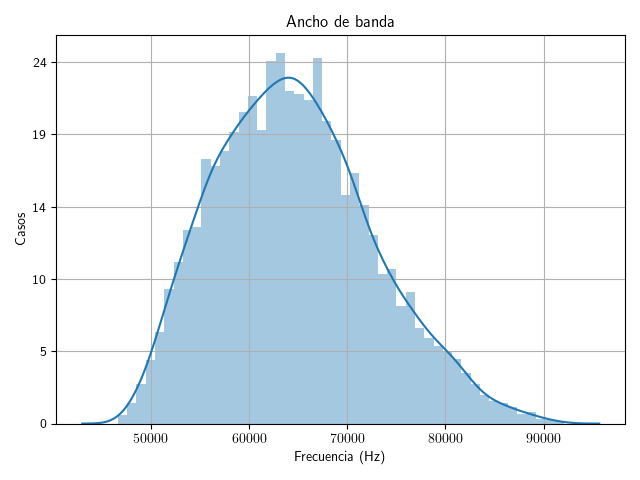
\includegraphics[scale = 0.5]{../Ejercicio2-DisenoDeCeldas/2CELDARAUCH/Informe/disp2.png}
    \caption{Histograma de Dispersión de f0 de la Segunda Etapa}
    \label{ej22dis1}
\end{figure}


\subsection{Análisis de Experimental}

\subsubsection{Respuesta en Frecuencia}

Realizando un análisis en frecuencia, superponiendo resultados teóricos, simulados y experimental se obtuvo el siguiente gráfico:

\begin{figure}[H]
    \centering
    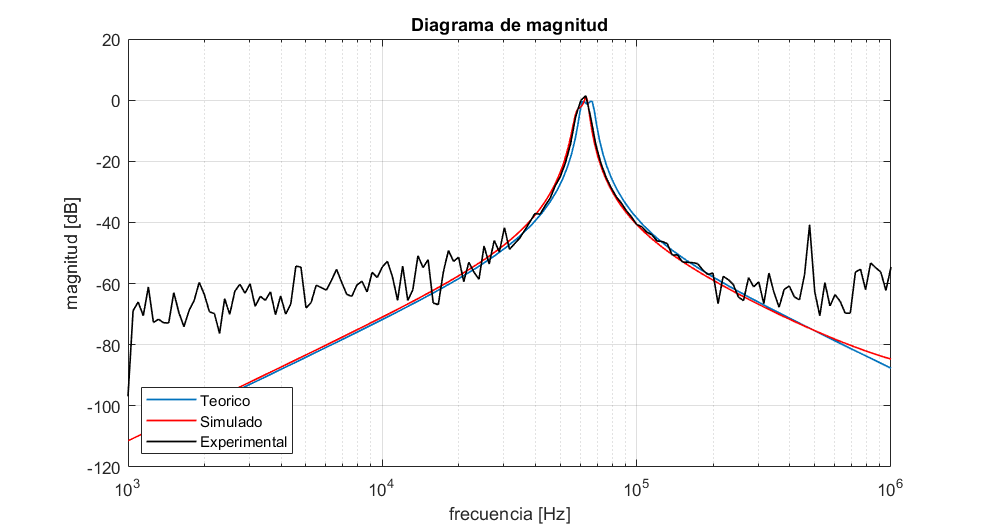
\includegraphics[scale = 0.6]{../Ejercicio2-DisenoDeCeldas/2CELDARAUCH/Informe/bodemag.png}
    % \includegraphics[scale = 0.6]{bodepha.png}
    % \caption{Respuesta en Frecuencia del Circuito}
    % \label{ej22bode}
\end{figure}
\begin{figure}[H]
    \centering
    \includegraphics[scale = 0.6]{../Ejercicio2-DisenoDeCeldas/2CELDARAUCH/Informe/bodepha.png}
    \caption{Respuesta en Frecuencia del Circuito}
    \label{ej22bode}
\end{figure}

En las frecuencias de interés, se puede observarse que se corresponden correctamente los valores medidos con los calculados, si bien con algunas leves diferencias debido a la tolerancia de los componentes pero se encuentra dentro de los resultados esperados. Es importante mencionar que como la atenuación a frecuencias lejanas al $f_0$, el circuito es susceptible al ruido, por lo que las mediciones se verán afectadas grandemente, creando oscilaciones indeseadas. Por otro lado, como se ve en la simulación y en la medición empírica, hay un salto de fase cuando $f>100kHz$, esta alteración es correspondiente al polo inducido por los amplificadores operacionales, dado que ahora no funcionan idealmente. 


\subsubsection{Impedancia de Entrada}

Como los amplificadores operacionales tienen una impedancia de entrada muy elevada, y no tener resistencias comparables para una correcta medición, se estudio la impedancia de entrada desde la simulación.

\begin{figure}[H]
    \centering
    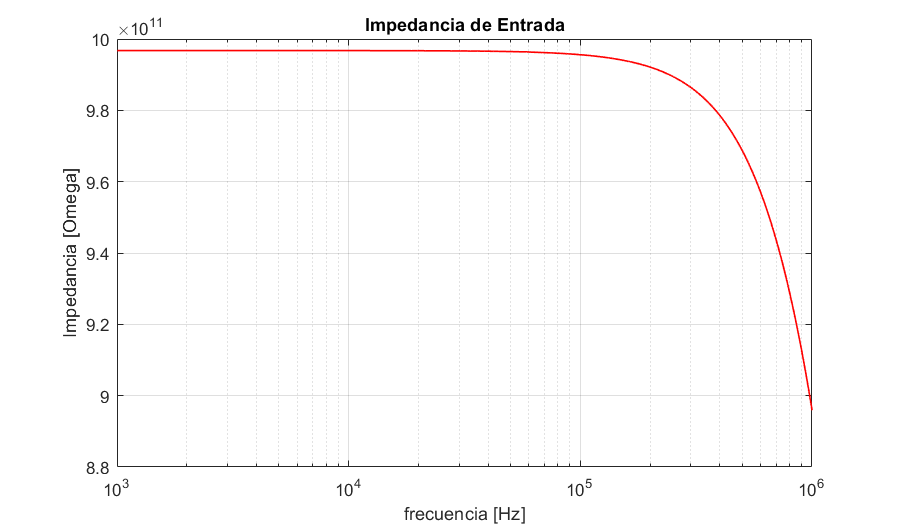
\includegraphics[scale = 0.5]{../Ejercicio2-DisenoDeCeldas/2CELDARAUCH/Informe/zin.png}
    \caption{Impedancia de Entrada Simulado}
    \label{ej22zin}
\end{figure}

\subsubsection{Rango Dinámico}

Para el calculo de rango dinámico, se utiliza la ganancia máxima del circuito experimentado $G = 1.45dB = 1.18$. La tensi\'on m\'axima a la salida ser\'a 6V teniendo en cuenta que la alimentaci\'on $\pm 9V$. Por lo tanto, para hallar la m\'axima tensión sera:

\begin{equation}
    V_i^{MAX} = \frac{V_o^{MAX}}{1.8} = 5.08V
\end{equation}

Luego, suponiendo que la  tensi\'on m\'inima distinguible es el piso de ruido, ya que por debajo de este nivel de tensi\'on no es posible distinguir entre la se\~nal y el ruido, se considera entonces $V_o^{MIN}=10mV$, por lo que resulta que:

\begin{equation}
    V_i^{MIN} = 10mV
\end{equation}

Entonces obtenemos el rango dinámico como:

\begin{equation}
    RD = 20log(\frac{V_i^{MAX}}{V_i^{MIN}})= 54.12dB
\end{equation}

\subsection{Conclusión}

Si bien los resultados resultaron ser similares a la esperado, es indispensable mencionar que no es filtro preciso ya que los componentes utilizados fueron con tolerancias mayores a $5\%$ y no se utilizo prestes debido a la falta de un milímetro para conocer el valor utilizado. Por otro lado, se debe destacar la cualidad de esta celda de Rauch que se pudo obtener un elevado valor de factor de calidad debido a la realimentación positiva y negativa, pero se debe también tener cuidado ya que si los valores del ciclo de realimentación positiva no están bien diseñados, el circuito podría oscilar.


\section{Introducción}

En este apartado se realiza un análisis de la celda denominada Sedra-Ghorab-Martin para posteriormente diseñar, sintetizar y analizar un filtro activo empleando dicha celda con valores recomendados por la cátedra. La principal fuente de información será el paper denominado Optimum configurations for Single-Amplifier Biquadratic Filters.

\section{Celda Sedra-Ghorab-Martin}

La celda Sedra-Ghorab-Martin (en adelante, celda SGB) es un circuito creado en el año 1980 por los miembros de IEEE cuyos nombres se reflejan en el nombre de la celda. Dicho circuito se basa en el circuito pasabanda de Deliyannis, que se reproduce a continuación. Los miembros propusieron dos circuitos bicuadráticos (con funciones transferencia de denominador y numerador de orden dos) que hacen uso del circuito pasabanda de Deliyannis, que se reproduce a continuación:

\begin{figure}[h]
	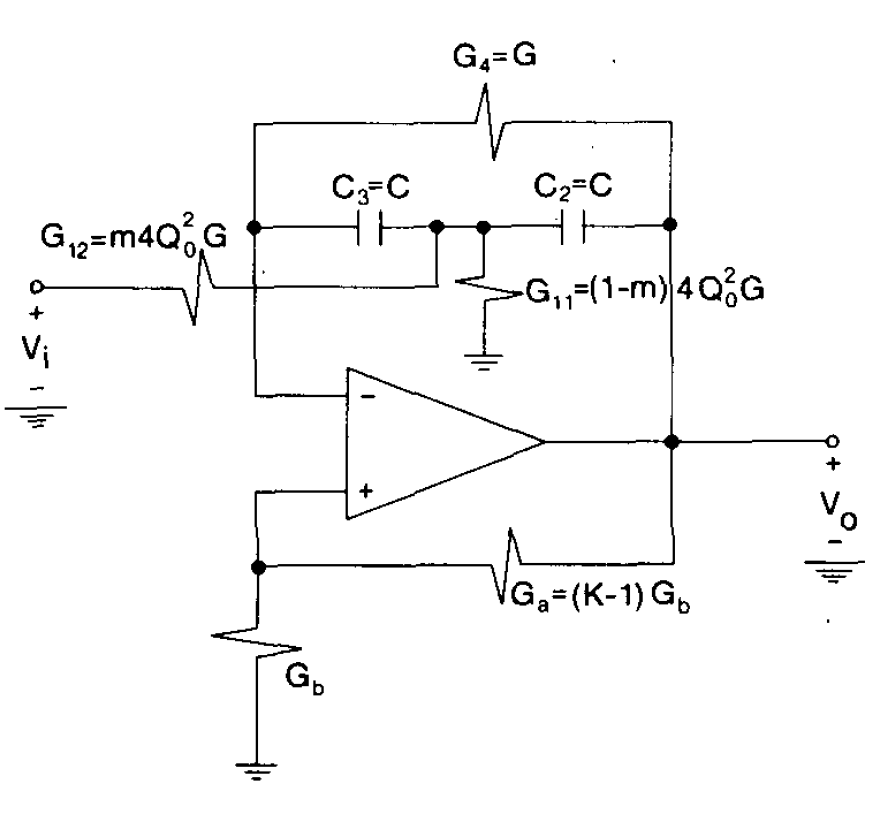
\includegraphics[width=0.8\textwidth]{../Ejercicio2-DisenoDeCeldas/3CeldaSedra/Imagenes/Celda Deliyannis.png}
	\centering
	\caption{Celda Pasabanda de Deliyannis}
	\label{Deliyannis pasabanda}
\end{figure}

Este circuito es posteriormente generalizado por Friend para poder construir cualquier tipo de configuración de filtro. El mismo se caracteriza por poseer una alta selectividad, empleando tanto realimentación positiva como negativa. Sin embargo, para poder sintetizar cualquier tipo de filtro es necesario cargar la red RC que se observa en la realimientación negativa del circuito, lo que hace poco realizable el diseño del mismo. Por otro lado, se encontró que realizando una transformación complementaria sobre el circuito de Deliyannis (esto es, intercambiando la salida del amplificador operacional por masa, y procediendo análogamente con la entrada inversora y no inversora del mismo) se deriva en el circuito de Sallen-Key manteniendo una realimentación positiva. Cabe destacar que esta transformación conserva la sensibilidad de los polos del circuito, pero no así con los ceros de transmisión del mismo. Aún así, se llegó a la conclusión de que es más ventajoso implementar las configuraciones de filtros en una celda Sallen-Key con realimentación positiva (exceptuando el caso de un filtro pasabanda).
En la siguiente figura se muestra como aplicando transformación complementaria y cambios en la red RC se obtienen los distintos circuitos:

\begin{figure}[h]
	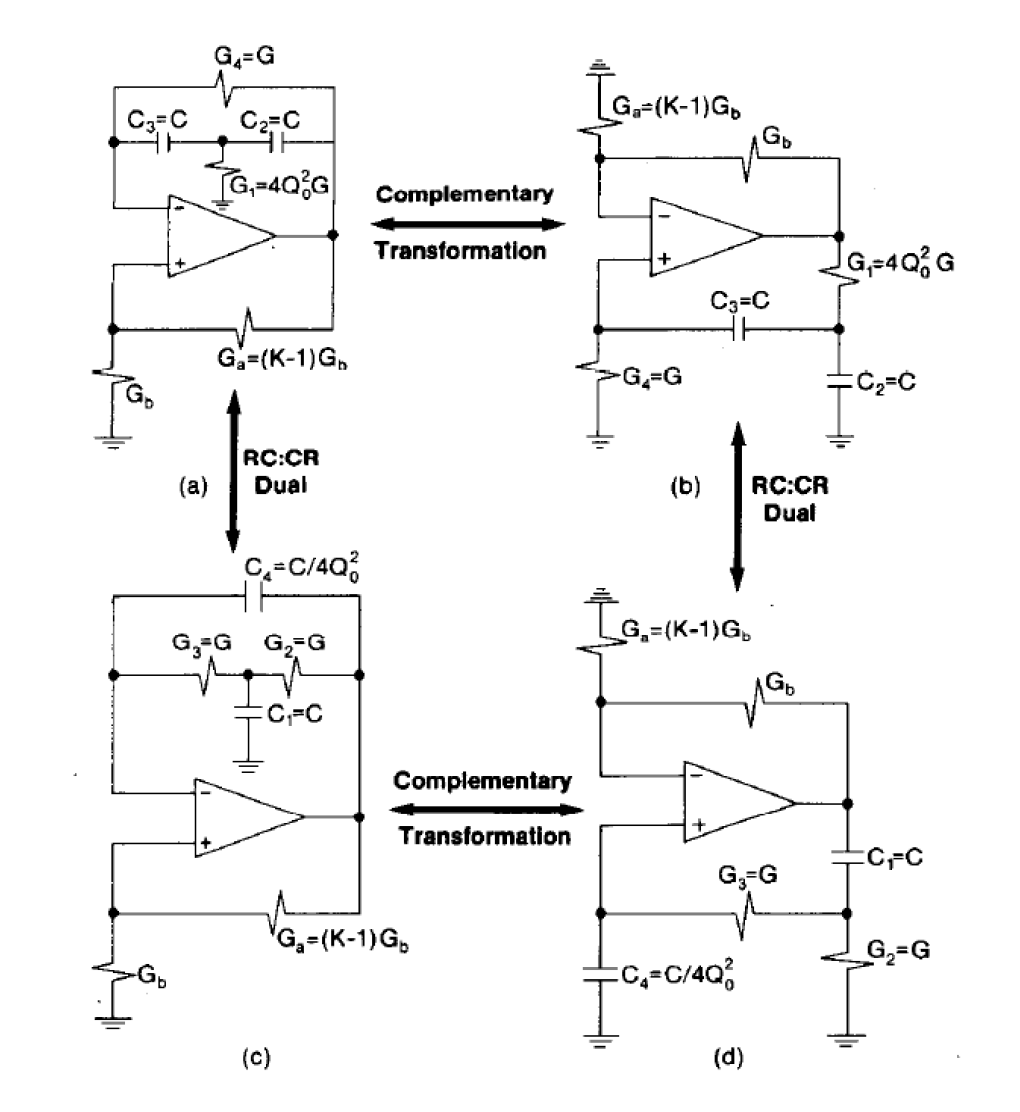
\includegraphics[width=0.8\textwidth]{../Ejercicio2-DisenoDeCeldas/3CeldaSedra/Imagenes/Transformaciones SGB.png}
	\centering
	\caption{Transformaciones de los circuitos }
	\label{transSGM}
\end{figure}

Los circuitos de la figura \ref{transSGM} (b) y \ref{transSGM} (d) son llamados EPF (Enhanced positive feedback), y son la base de la celda SGB. Esta característica esta dada por un coeficiente K $>$ 1. La ecuación que describe el comportamiento de los cuatro circuitos mostrado anteriormente es:

\begin{equation}
	\frac{C}{G} = \frac{2Q_0}{\omega_0}
	\label{eq C/G}
\end{equation}

\begin{equation}
	K - 1 = \frac{1}{2Q_0^2} (1-\frac{Q_0}{Q})
	\label{eq K-1}
\end{equation}

Donde $Q_0$ es un parámetro de diseño que cumple $Q>Q_0$. De esta forma, los circuitos del tipo EPF permiten
implementar filtros con la siguiente función transferencia de segundo orden:

\begin{equation}
	H(s) = \frac{n_2 s^2 + n_1 s + n_0}{s^2 + s (\frac{\omega_0}{Q}) + \omega_0^2}
	\label{eq transferencia general}
\end{equation}

Siendo los coeficientes $n_i$ los ceros de transmision que determinan el tipo de filtro que se implementa. Para poder lograr esto sin afectar la ubicacion de los polos se necesita que aquellos componentes que se encuentren conectados a masa sean desconectados de la misma, total o parcialmente. De esta forma se obtienen los circcuitos HPB(High-Pass Biquad) y LPB(Low-Pass Biquad) que se mostrarán a continuación:

\begin{figure}[h]
	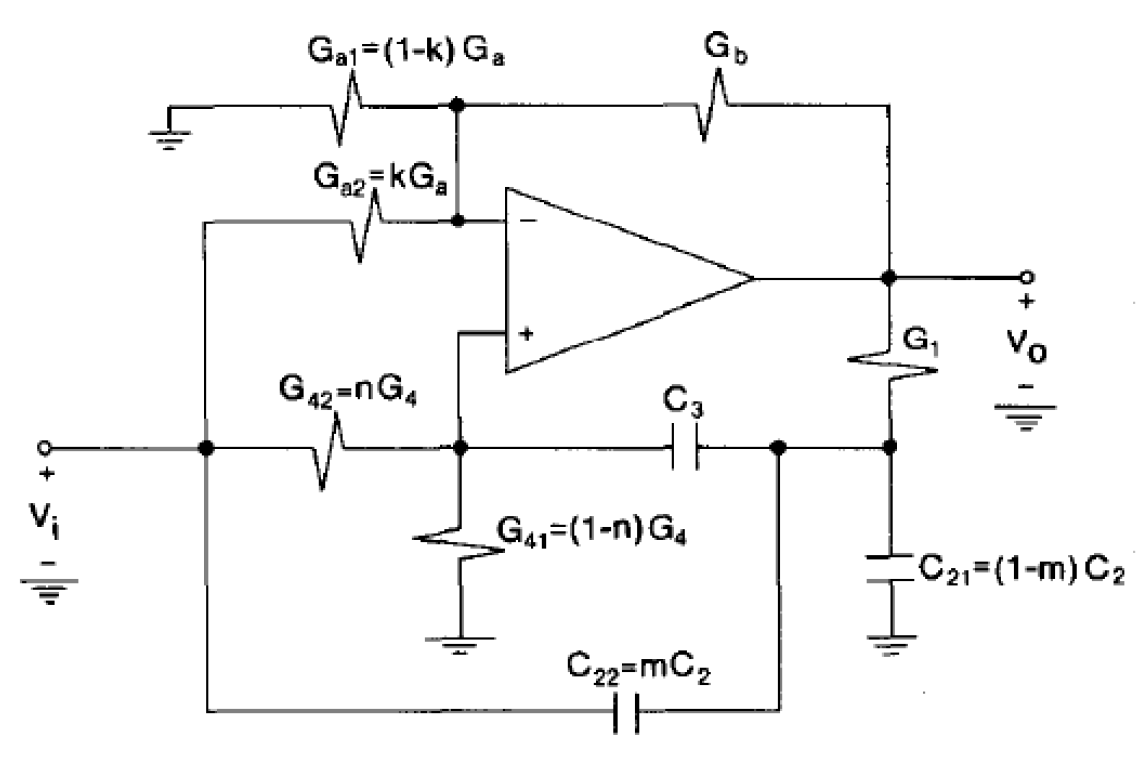
\includegraphics[width=0.6\textwidth]{../Ejercicio2-DisenoDeCeldas/3CeldaSedra/Imagenes/HP biquad.png}
	\centering
	\caption{High-pass biquad}
	\label{HPB}
\end{figure}

\begin{figure}[h]
	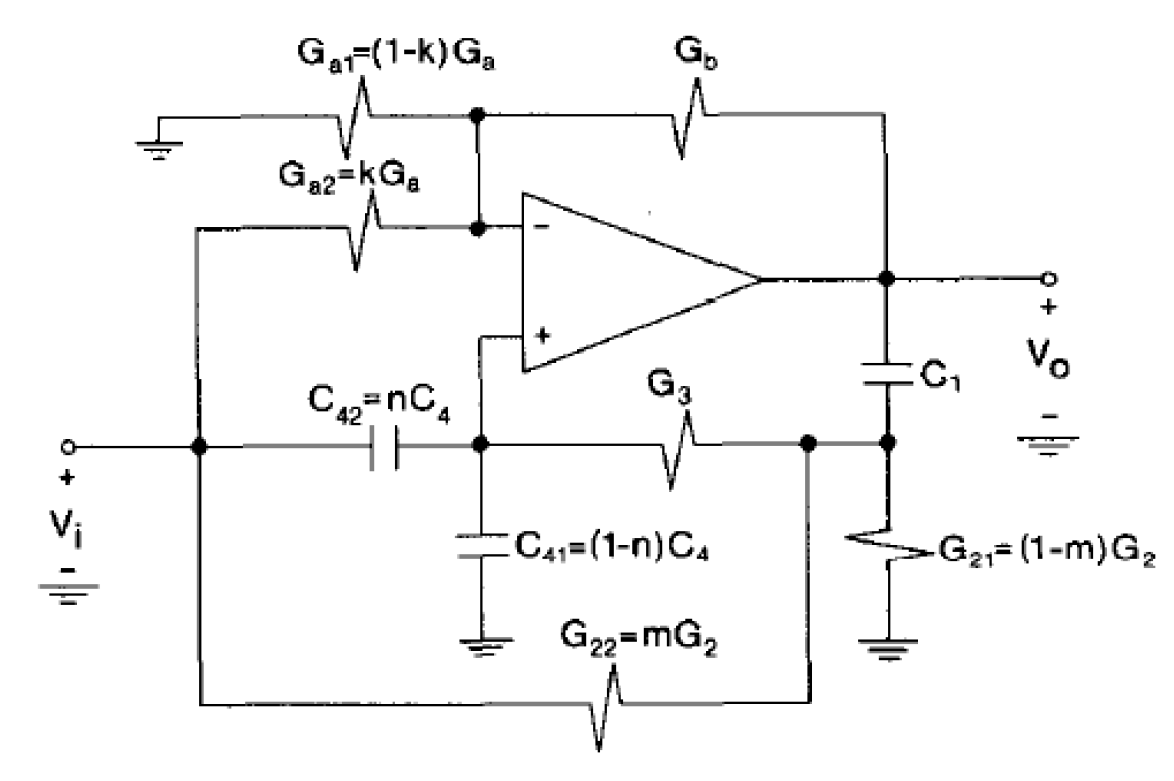
\includegraphics[width=0.6\textwidth]{../Ejercicio2-DisenoDeCeldas/3CeldaSedra/Imagenes/LP biquad.png}
	\centering
	\caption{Low-pass biquad}
	\label{LPB}
\end{figure}

\section{Análisis matemático}

A partir de la ecuacion \ref{eq transferencia general} se puede ver que se deben hallar los coeficientes $n_i$, los cuales están determinados por el tipo de circuito que se desea implementar. En nuestro caso se trata de un HPB por lo que las ecuaciones serán las siguientes:

\subsubsection*{Caso HPB}
\begin{equation}
	n_0= \frac{G_1(G_{41}+G_{42} )}{C_3 ( C_{21} + C_{22} )} \left( \frac{G_{42}}{G_{41}+G_{42}} . \frac{G_{a1}+G_{a2}+G_{b}}{G_b} - \frac{G_{a2}}{G_b} \right)
	\label{coef n0 HPB}
\end{equation}

\begin{equation}
	n_1 = \frac{G_{a1}+G_{a2}+G_b}{G_b} . G_{42}. \left( \frac{1}{C_{21} + C_{22}} + \frac{1}{C_3} \right) - \frac{G_{a2}}{G_b} \left[ \frac{G_1}{C_{21} + C_{22}} + (G_{41}+G_{42}) \left( \frac{1}{C_{21} + C_{22}} + \frac{1}{C_3} \right) \right]
	\label{coef n1 HPB}
\end{equation}

\begin{equation}
	n_2 = \frac{G_{a1}+G_{a2}+G_b}{G_b} . \frac{C_{22}}{C_{21} + C_{22}} - \frac{G_{a2}}{G_b}
	\label{coef n2 HPB}
\end{equation}


\subsubsection*{Caso LPB}

\begin{equation}
	n_0= \frac{G_3(G_{21}+G_{22} )}{C_1 ( C_{41} + C_{42} )} \left( \frac{G_{22}}{G_{21}+G_{22}} . \frac{G_{a1}+G_{a2}+G_{b}}{G_b} - \frac{G_{a2}}{G_b} \right)
	\label{coef n0 LPB}
\end{equation}

\begin{equation}
	n_1 = \frac{G_{a1}+G_{a2}+G_b}{G_b}. G_{42}. \frac{C_{42}}{C_{41}+C_{42}} . \frac{G_{21} + G_{22} + G_3}{C_1} - \frac{G_{a2}}{G_b} . \left( \frac{G_3}{C_{41} + C_{42}} + \frac{G_{21}+G_{22} + G_3}{C_1}\right)
	\label{coef n1 LPB}
\end{equation}

\begin{equation}
	n_2 = \frac{G_{a1}+G_{a2}+G_b}{G_b} . \frac{C_{22}}{C_{21} + C_{22}} - \frac{G_{a2}}{G_b}
	\label{coef n2 LPB}
\end{equation}

En pocas palabras hay que tenes en cuenta los sub-índices en las ecuaciones ya que son complementarias entre si. Para los  denominadores se toman las siguientes ecuaciones características:

\subsubsection*{Caso HPB}

\begin{equation}
\omega_0 = \frac{G_1 ( G_{41} + G_{42} )}{C_3 ( C_{21} + C_{22} ) }
\label{w0 HPB}
\end{equation}

\begin{equation}
\frac{\omega_0}{Q} = (G_{41}+G_{42}). \left( \frac{1}{C_{21} + C_{22}} + \frac{1}{C_3} \right) - \frac{G_1}{C_{21} + C_{22}} . \frac{G_{a1}+G_{a2}}{G_b}
\label{w/Q HPB}
\end{equation}

\subsubsection*{Caso LPB}

\begin{equation}
\omega_0 = \frac{G_3 ( G_{21} + G_{22} )}{C_1 ( C_{41} + C_{42} ) }
\label{w0 LPB}
\end{equation}

\begin{equation}
\frac{\omega_0}{Q} = \frac{G_{21} + G_{22} + G_3}{C_1} - \frac{G_3}{G_{41}+G_{42}} . \frac{G_{a1}+G_{a2}}{G_b}
\label{w/Q LPB}
\end{equation}

\subsection{Sensibilidades}

La sensibilidades del circuito se pueden diferenciar a grandes rasgos por dos muy importantes, las que corresponden a componentes pasivos (resistores y capacitores) y las que corresponden a componentes activos (amplificadores operacionales). El valor de $Q_0$ determina el balance entre los dos tipos de sensibilidades, por lo que su elección debe ser llevada a cabo considerando los valores de dispersión de ambos grupos de componentes. La ecuación que caracteriza $Q_0$ es la siguiente:

\begin{equation}
Q_0 = \left[ |A(s_0)| ^2 . \frac{8\sigma_R^2 + \sigma_C^2}{8\sigma
_A^2} \right] ^\frac{1}{4}
\label{eq Q0}
\end{equation}
Donde $\sigma_R$ es la variación de los resistores, $\sigma_C$ es la variación de los capacitores y $\sigma_A$ es la variación de la ganancia del Op-Amp. Mientras que $A(s_0)$ es la ganancia del amplificador operacional en la frecuencia nominal del polo s0, siendo esta
última:

\begin{equation}
s_0 = -\frac{\omega_0}{2Q} + j\omega_0 \sqrt{1-\frac{1}{4Q^2}}
\label{eq s0}
\end{equation}

A partir de estas ecuaciones es posible determinar las sensibilidades con respecto a cada componente en ambos casos, siendo las sensibilidades correspondientes las mostradas en la siguiente tabla:

\begin{table}[h]
\begin{tabular}{@{}|c|c|c|c|c|c|@{}}
\toprule
\textbf{HPB} & \textbf{$\omega_0$} & \textbf{Q}                         & \textbf{LPB} & \textbf{$\omega_0$} & \textbf{Q}                         \\ 
\midrule
$R_1$         & $-\frac{1}{2}$                      & $-(\frac{Q}{Q_0} - \frac{1}{2})$    & $C_1$         & $-\frac{1}{2}$                      & $-(\frac{Q}{Q_0} - \frac{1}{2})$    \\
$C_2$         & $-\frac{1}{2}$                      & $-\frac{1}{2} (\frac{Q}{Q_0} - 1)$ & $R_2$         & $-\frac{1}{2}$                      & $-\frac{1}{2} (\frac{Q}{Q_0} - 1)$ \\
$C_3$         & $-\frac{1}{2}$                      & $\frac{1}{2} (\frac{Q}{Q_0} - 1)$  & $R_3$          & $-\frac{1}{2}$                      & $\frac{1}{2} (\frac{Q}{Q_0} - 1)$  \\
$R_4$         & $-\frac{1}{2}$                      & $(\frac{Q}{Q_0} - \frac{1}{2})$     & $C_4$         & $-\frac{1}{2}$                      & $(\frac{Q}{Q_0} - \frac{1}{2})$     \\
$R_a$         & 0                                   & $- (\frac{Q}{Q_0} - 1)$            & $R_a$         & 0                                   & $- (\frac{Q}{Q_0} - 1)$            \\
$R_b$         & 0                                   & $ (\frac{Q}{Q_0} - 1)$             & $R_b$         & 0                                   & $ (\frac{Q}{Q_0} - 1)$            
\end{tabular}
\centering
\caption{Tabla de sensibilidades}
\label{tabla sensibilidades}
\end{table}

\subsection{Aproximación del filtro}

La cátedra nos dispuso de una plantilla para implementar un filtro pasa-altos activo. Para tener un margen de tolerancia se usaron valores más restrictivos mostrados en la siguiente tabla:

\begin{table}[h]
\begin{tabular}{@{}|c|c|c|@{}}
\toprule
\textbf{Parámetro} & \textbf{Valor propuesto} & \textbf{Valor elegido} \\ \midrule
$f_a$              & $13,3k\Omega$              & $13,5k\Omega$            \\
$f_p$              & $26,6k\Omega$              & $27k\Omega$              \\
$A_a$              & $40dB$                     & $45dB$      			   \\
$A_p$              & $2dB$                      & $1,5dB$				   \\
$Z_{in}$           & $\geq50k\Omega$            & $\geq50k\Omega$           
\end{tabular}
\centering
\caption{Valores propuesto por la cátedra y elegido por nosotros}
\label{tabla componentes}
\end{table}

El primer paso para el diseño del mismo es normalizar la plantilla a una de un pasa-altos, con frecuencia angular pasante unitaria ($\omega_p =1$). Una vez hecho esto se procede a aplicar la aproximación de Cauer sobre dicha plantilla.
La aproximación de Cauer es una aproximación por funciones elípticas, con riple constante tanto en la banda de paso como la de atenuación. 



\subsection{Etapa I}

\subsection{Etapa II}

